\hypertarget{Predict_8c}{
\section{Predict.c File Reference}
\label{Predict_8c}\index{Predict.c@{Predict.c}}
}
{\tt \#include \char`\"{}party.h\char`\"{}}\par


Include dependency graph for Predict.c:\begin{figure}[H]
\begin{center}
\leavevmode
\includegraphics[width=160pt]{Predict_8c__incl}
\end{center}
\end{figure}
\subsection*{Functions}
\begin{CompactItemize}
\item 
void \hyperlink{Predict_8c_daf8a0eb8790ebf14f0e265de164d50e}{C\_\-splitnode} (SEXP node, SEXP learnsample, SEXP control)
\item 
SEXP \hyperlink{Predict_8c_dcd61d38c7c43d241d09a600b70fe3c5}{C\_\-get\_\-node} (SEXP subtree, SEXP newinputs, double mincriterion, int numobs)
\item 
SEXP \hyperlink{Predict_8c_dec31e3aa985e0af16ccaeac31237640}{R\_\-get\_\-node} (SEXP subtree, SEXP newinputs, SEXP mincriterion, SEXP numobs)
\item 
SEXP \hyperlink{Predict_8c_201fdee9dc7e3e71e90ea6609ed353cb}{C\_\-get\_\-nodebynum} (SEXP subtree, int nodenum)
\item 
SEXP \hyperlink{Predict_8c_4a30a8aa916f294059b6e2cbcb9e29d5}{R\_\-get\_\-nodebynum} (SEXP subtree, SEXP nodenum)
\item 
SEXP \hyperlink{Predict_8c_c4f4e806a78c376b13802ed2cf1e7b65}{C\_\-get\_\-prediction} (SEXP subtree, SEXP newinputs, double mincriterion, int numobs)
\item 
SEXP \hyperlink{Predict_8c_cbb3e45d03e1b544c94bf639b191a953}{C\_\-get\_\-nodeweights} (SEXP subtree, SEXP newinputs, double mincriterion, int numobs)
\item 
int \hyperlink{Predict_8c_d9d49b6a210f5c09a2a1d1aa496859ce}{C\_\-get\_\-node\-ID} (SEXP subtree, SEXP newinputs, double mincriterion, int numobs)
\item 
SEXP \hyperlink{Predict_8c_c0668d268fe5a4bad29fbf4ead39c526}{R\_\-get\_\-node\-ID} (SEXP tree, SEXP newinputs, SEXP mincriterion)
\item 
void \hyperlink{Predict_8c_ac36eff20575604b5d7558d512601d64}{C\_\-predict} (SEXP tree, SEXP newinputs, double mincriterion, SEXP ans)
\item 
SEXP \hyperlink{Predict_8c_9a5170a24bc00b727527b80cec5ca60a}{R\_\-predict} (SEXP tree, SEXP newinputs, SEXP mincriterion)
\item 
void \hyperlink{Predict_8c_8964e7493ed9cb96c271b168b721e329}{C\_\-getpredictions} (SEXP tree, SEXP where, SEXP ans)
\item 
SEXP \hyperlink{Predict_8c_a508a31f1fd7cd3668ad81eb0d00dd66}{R\_\-getpredictions} (SEXP tree, SEXP where)
\item 
void \hyperlink{Predict_8c_1e3892117a14a178e707acf56ab56f5c}{C\_\-getweights} (SEXP tree, SEXP where, SEXP ans)
\item 
SEXP \hyperlink{Predict_8c_f255340d550e1387709b1674467c31b9}{R\_\-getweights} (SEXP tree, SEXP where)
\item 
void \hyperlink{Predict_8c_830785cf09ef008b28bd8577feb6d06b}{C\_\-weights} (SEXP tree, SEXP newinputs, double mincriterion, SEXP ans)
\item 
SEXP \hyperlink{Predict_8c_0f24ac195825953e630d3386b4d98f97}{R\_\-weights} (SEXP tree, SEXP newinputs, SEXP mincriterion)
\item 
SEXP \hyperlink{Predict_8c_20dd01c361767edbfc62abf55ce30ff1}{R\_\-predict\-RF} (SEXP forest, SEXP newinputs, SEXP mincriterion, SEXP oobpred)
\item 
SEXP \hyperlink{Predict_8c_a4f23088af5379408f00d3809656d0da}{R\_\-predict\-RF2} (SEXP forest, SEXP response, SEXP newinputs, SEXP mincriterion, SEXP oobpred)
\item 
SEXP \hyperlink{Predict_8c_b1c6e1c0c34af27c7f587b53deb4dc4f}{R\_\-predict\-RF\_\-weights} (SEXP forest, SEXP newinputs, SEXP mincriterion, SEXP oobpred)
\end{CompactItemize}


\subsection{Detailed Description}
Node splitting and prediction

\begin{Desc}
\item[Author:]\begin{Desc}
\item[Author]hothorn \end{Desc}
\end{Desc}
\begin{Desc}
\item[Date:]\begin{Desc}
\item[Date]2007-02-02 11:22:45 +0100 (Fri, 02 Feb 2007) \end{Desc}
\end{Desc}


Definition in file \hyperlink{Predict_8c-source}{Predict.c}.

\subsection{Function Documentation}
\hypertarget{Predict_8c_dcd61d38c7c43d241d09a600b70fe3c5}{
\index{Predict.c@{Predict.c}!C_get_node@{C\_\-get\_\-node}}
\index{C_get_node@{C\_\-get\_\-node}!Predict.c@{Predict.c}}
\subsubsection[C\_\-get\_\-node]{\setlength{\rightskip}{0pt plus 5cm}SEXP C\_\-get\_\-node (SEXP {\em subtree}, SEXP {\em newinputs}, double {\em mincriterion}, int {\em numobs})}}
\label{Predict_8c_dcd61d38c7c43d241d09a600b70fe3c5}


Get the terminal node for obs. number `numobs' of `newinputs' \par
 \begin{Desc}
\item[Parameters:]
\begin{description}
\item[{\em subtree}]a tree \item[{\em newinputs}]an object of class `Variable\-Frame' \item[{\em mincriterion}]overwrites mincriterion used for tree growing \item[{\em numobs}]observation number \end{description}
\end{Desc}
\begin{Desc}
\item[\hyperlink{todo__todo000002}{Todo}]handle surrogate splits \end{Desc}


Definition at line 120 of file Predict.c.

References C\_\-i\_\-in\_\-set(), get\_\-missings(), get\_\-variable(), has\_\-missings(), S3get\_\-leftnode(), S3get\_\-maxcriterion(), S3get\_\-nodeterminal(), S3get\_\-nodeweights(), S3get\_\-primarysplit(), S3get\_\-rightnode(), S3get\_\-splitpoint(), S3get\_\-surrogatesplits(), S3get\_\-toleft(), S3get\_\-variable\-ID(), and S3is\_\-ordered().

Referenced by C\_\-get\_\-node\-ID(), C\_\-get\_\-nodeweights(), C\_\-get\_\-prediction(), and R\_\-get\_\-node().

Here is the call graph for this function:\begin{figure}[H]
\begin{center}
\leavevmode
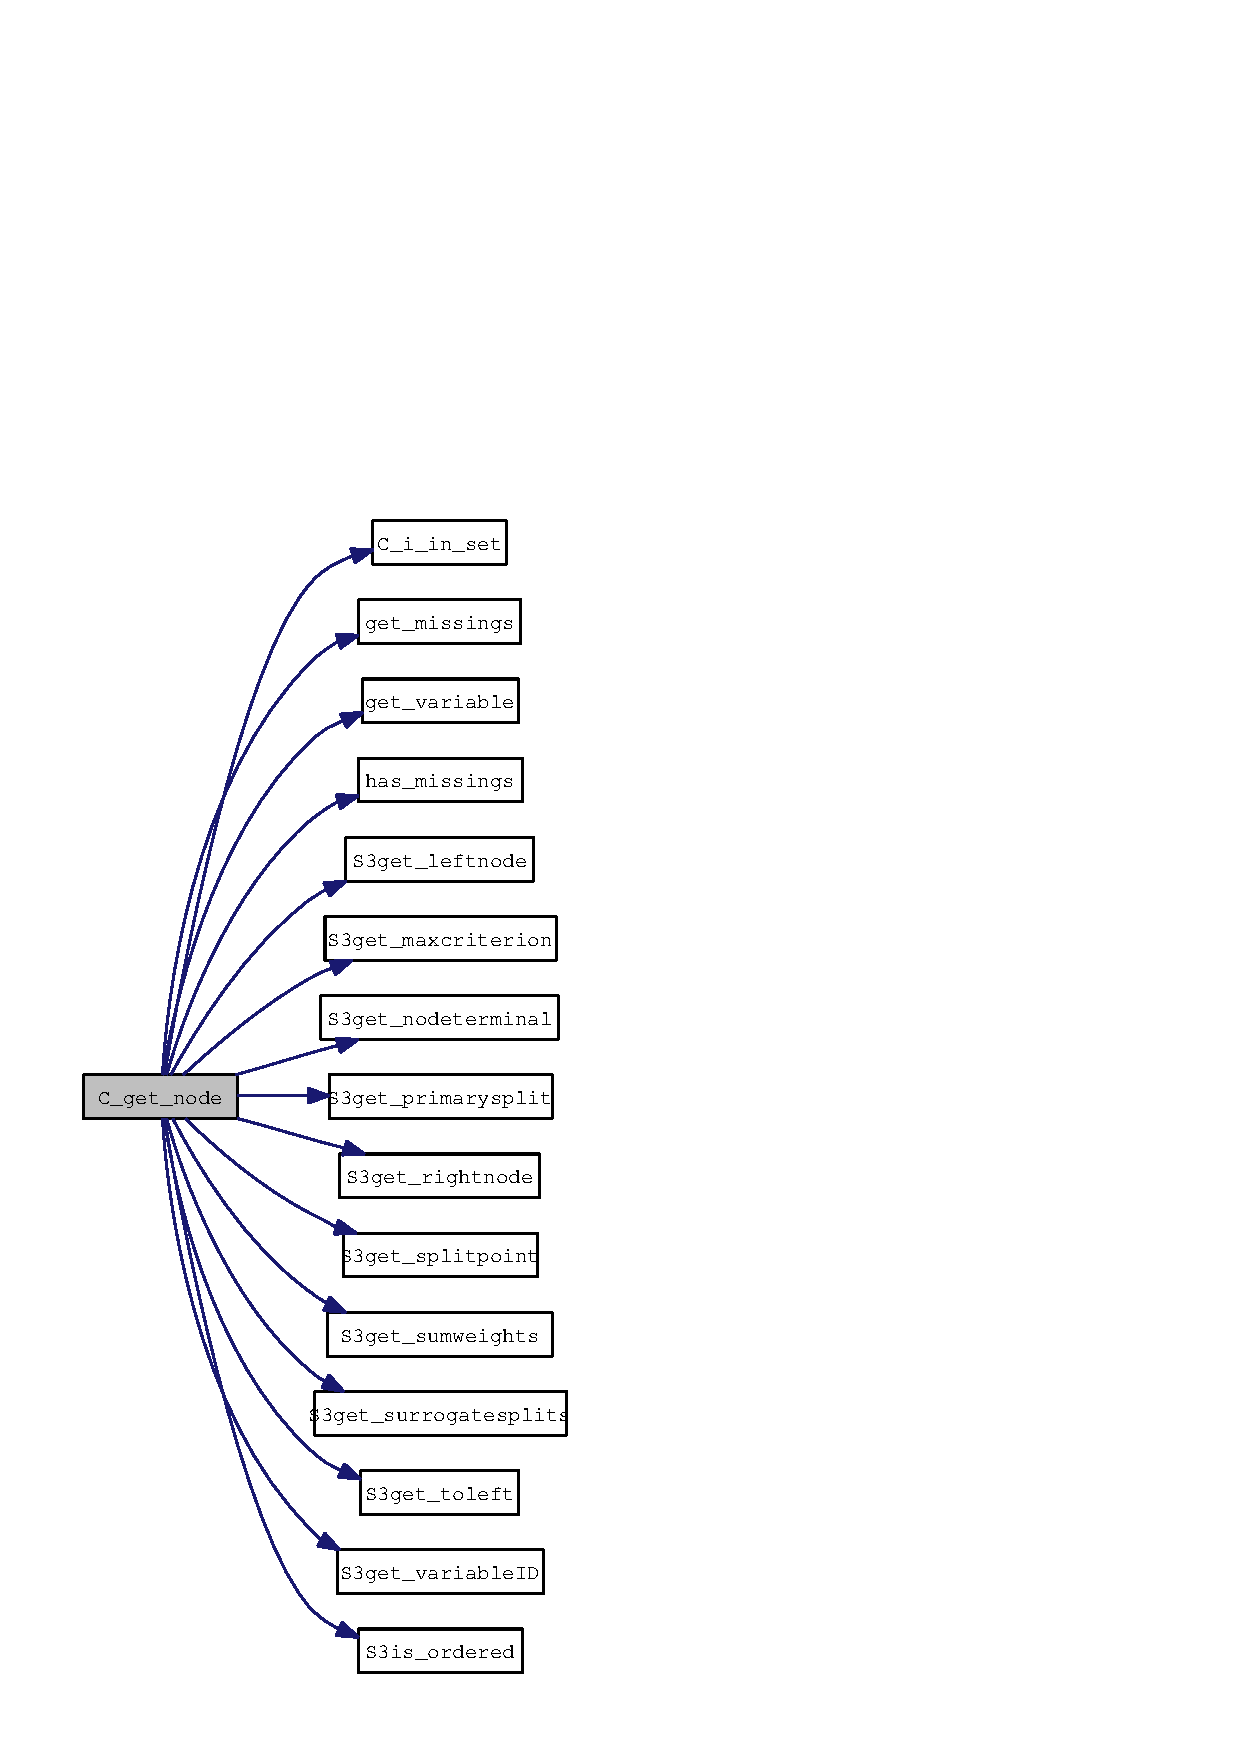
\includegraphics[width=186pt]{Predict_8c_dcd61d38c7c43d241d09a600b70fe3c5_cgraph}
\end{center}
\end{figure}
\hypertarget{Predict_8c_201fdee9dc7e3e71e90ea6609ed353cb}{
\index{Predict.c@{Predict.c}!C_get_nodebynum@{C\_\-get\_\-nodebynum}}
\index{C_get_nodebynum@{C\_\-get\_\-nodebynum}!Predict.c@{Predict.c}}
\subsubsection[C\_\-get\_\-nodebynum]{\setlength{\rightskip}{0pt plus 5cm}SEXP C\_\-get\_\-nodebynum (SEXP {\em subtree}, int {\em nodenum})}}
\label{Predict_8c_201fdee9dc7e3e71e90ea6609ed353cb}


Get the node with node\-ID `nodenum' \par
 \begin{Desc}
\item[Parameters:]
\begin{description}
\item[{\em subtree}]a tree \item[{\em nodenum}]a node\-ID \end{description}
\end{Desc}


Definition at line 250 of file Predict.c.

References S3get\_\-leftnode(), S3get\_\-node\-ID(), S3get\_\-nodeterminal(), and S3get\_\-rightnode().

Referenced by C\_\-getpredictions(), C\_\-getweights(), R\_\-get\_\-nodebynum(), R\_\-predict\-RF(), R\_\-predict\-RF2(), and R\_\-predict\-RF\_\-weights().

Here is the call graph for this function:\begin{figure}[H]
\begin{center}
\leavevmode
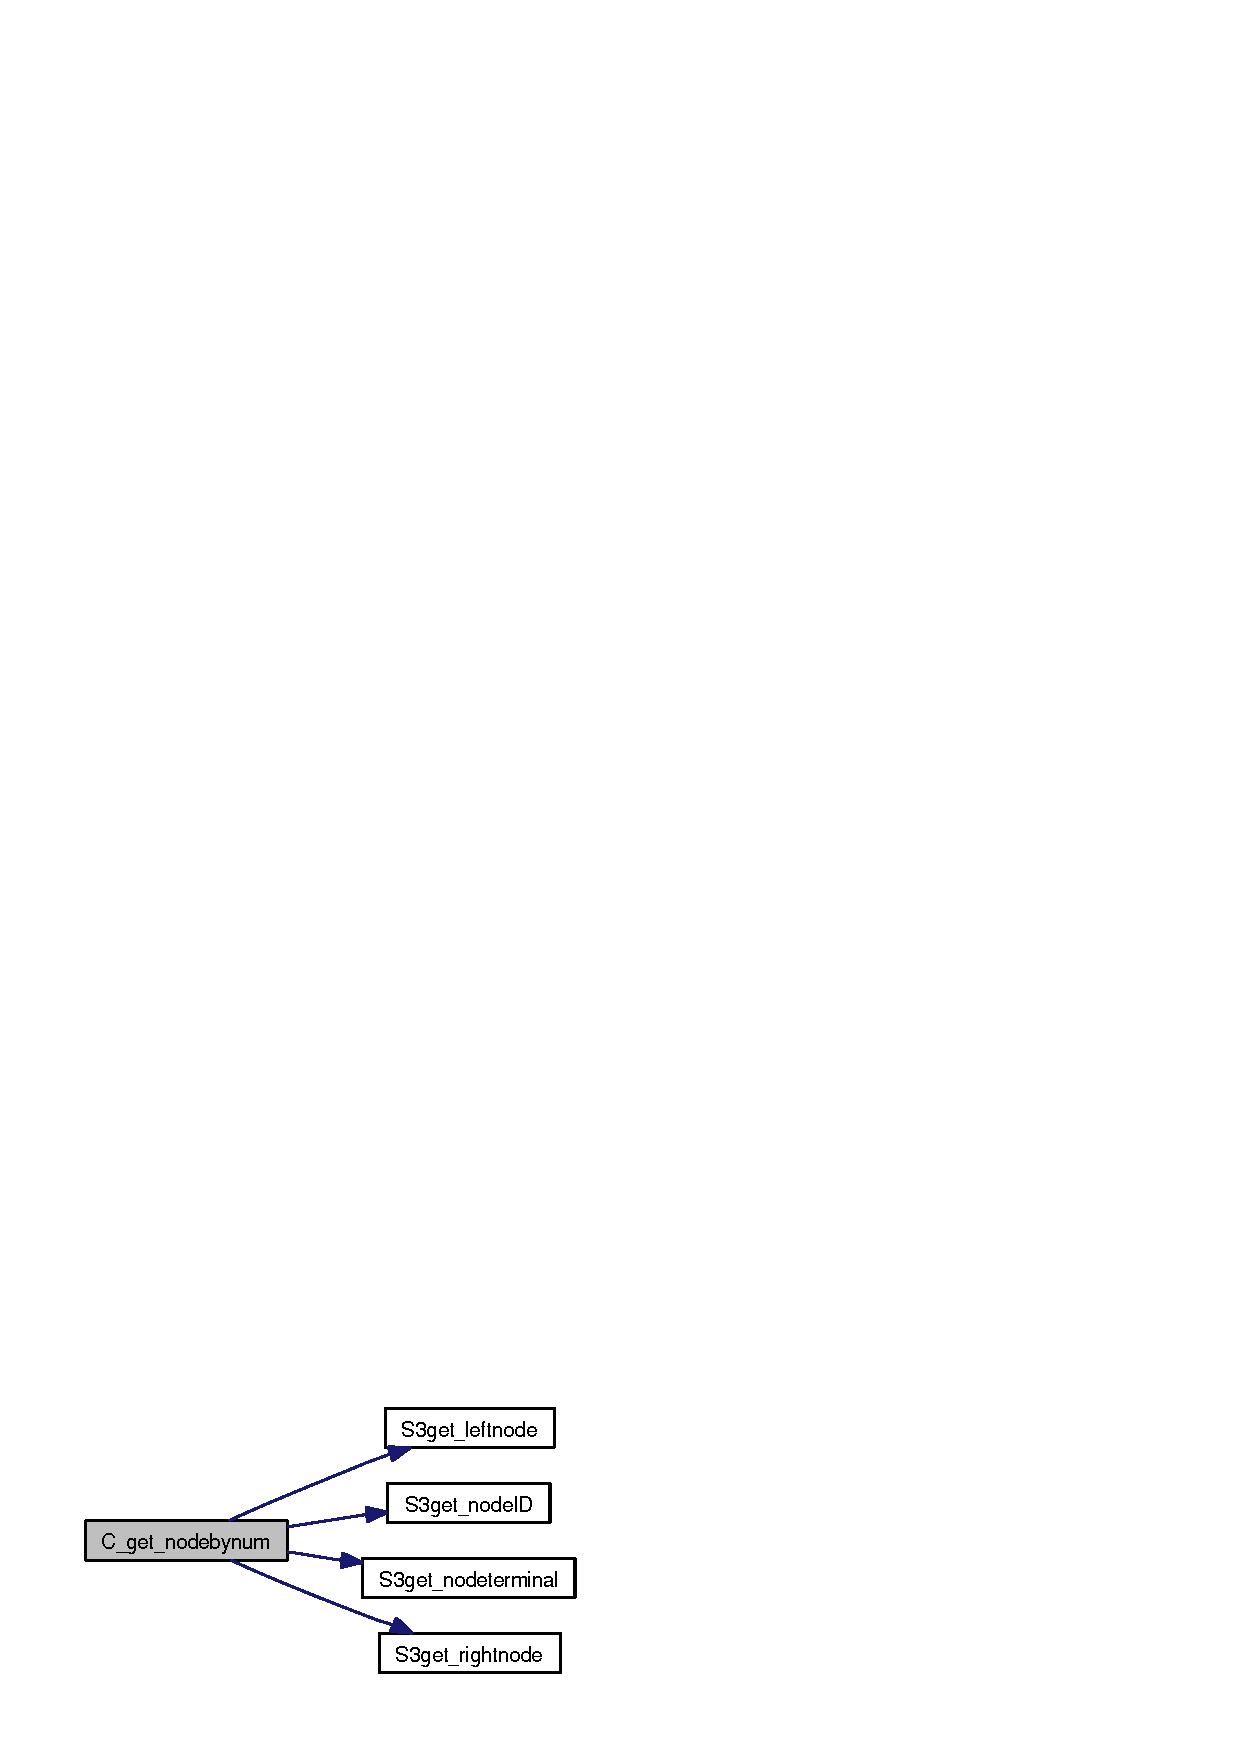
\includegraphics[width=140pt]{Predict_8c_201fdee9dc7e3e71e90ea6609ed353cb_cgraph}
\end{center}
\end{figure}
\hypertarget{Predict_8c_d9d49b6a210f5c09a2a1d1aa496859ce}{
\index{Predict.c@{Predict.c}!C_get_nodeID@{C\_\-get\_\-nodeID}}
\index{C_get_nodeID@{C\_\-get\_\-nodeID}!Predict.c@{Predict.c}}
\subsubsection[C\_\-get\_\-nodeID]{\setlength{\rightskip}{0pt plus 5cm}int C\_\-get\_\-node\-ID (SEXP {\em subtree}, SEXP {\em newinputs}, double {\em mincriterion}, int {\em numobs})}}
\label{Predict_8c_d9d49b6a210f5c09a2a1d1aa496859ce}


Get the node\-ID for a new observation \par
 \begin{Desc}
\item[Parameters:]
\begin{description}
\item[{\em subtree}]a tree \item[{\em newinputs}]an object of class `Variable\-Frame' \item[{\em mincriterion}]overwrites mincriterion used for tree growing \item[{\em numobs}]observation number \end{description}
\end{Desc}


Definition at line 314 of file Predict.c.

References C\_\-get\_\-node(), and S3get\_\-node\-ID().

Referenced by R\_\-get\_\-node\-ID(), R\_\-predict\-RF(), R\_\-predict\-RF2(), and R\_\-predict\-RF\_\-weights().

Here is the call graph for this function:\begin{figure}[H]
\begin{center}
\leavevmode
\includegraphics[width=249pt]{Predict_8c_d9d49b6a210f5c09a2a1d1aa496859ce_cgraph}
\end{center}
\end{figure}
\hypertarget{Predict_8c_cbb3e45d03e1b544c94bf639b191a953}{
\index{Predict.c@{Predict.c}!C_get_nodeweights@{C\_\-get\_\-nodeweights}}
\index{C_get_nodeweights@{C\_\-get\_\-nodeweights}!Predict.c@{Predict.c}}
\subsubsection[C\_\-get\_\-nodeweights]{\setlength{\rightskip}{0pt plus 5cm}SEXP C\_\-get\_\-nodeweights (SEXP {\em subtree}, SEXP {\em newinputs}, double {\em mincriterion}, int {\em numobs})}}
\label{Predict_8c_cbb3e45d03e1b544c94bf639b191a953}


Get the weights for a new observation \par
 \begin{Desc}
\item[Parameters:]
\begin{description}
\item[{\em subtree}]a tree \item[{\em newinputs}]an object of class `Variable\-Frame' \item[{\em mincriterion}]overwrites mincriterion used for tree growing \item[{\em numobs}]observation number \end{description}
\end{Desc}


Definition at line 299 of file Predict.c.

References C\_\-get\_\-node(), and S3get\_\-nodeweights().

Referenced by C\_\-weights().

Here is the call graph for this function:\begin{figure}[H]
\begin{center}
\leavevmode
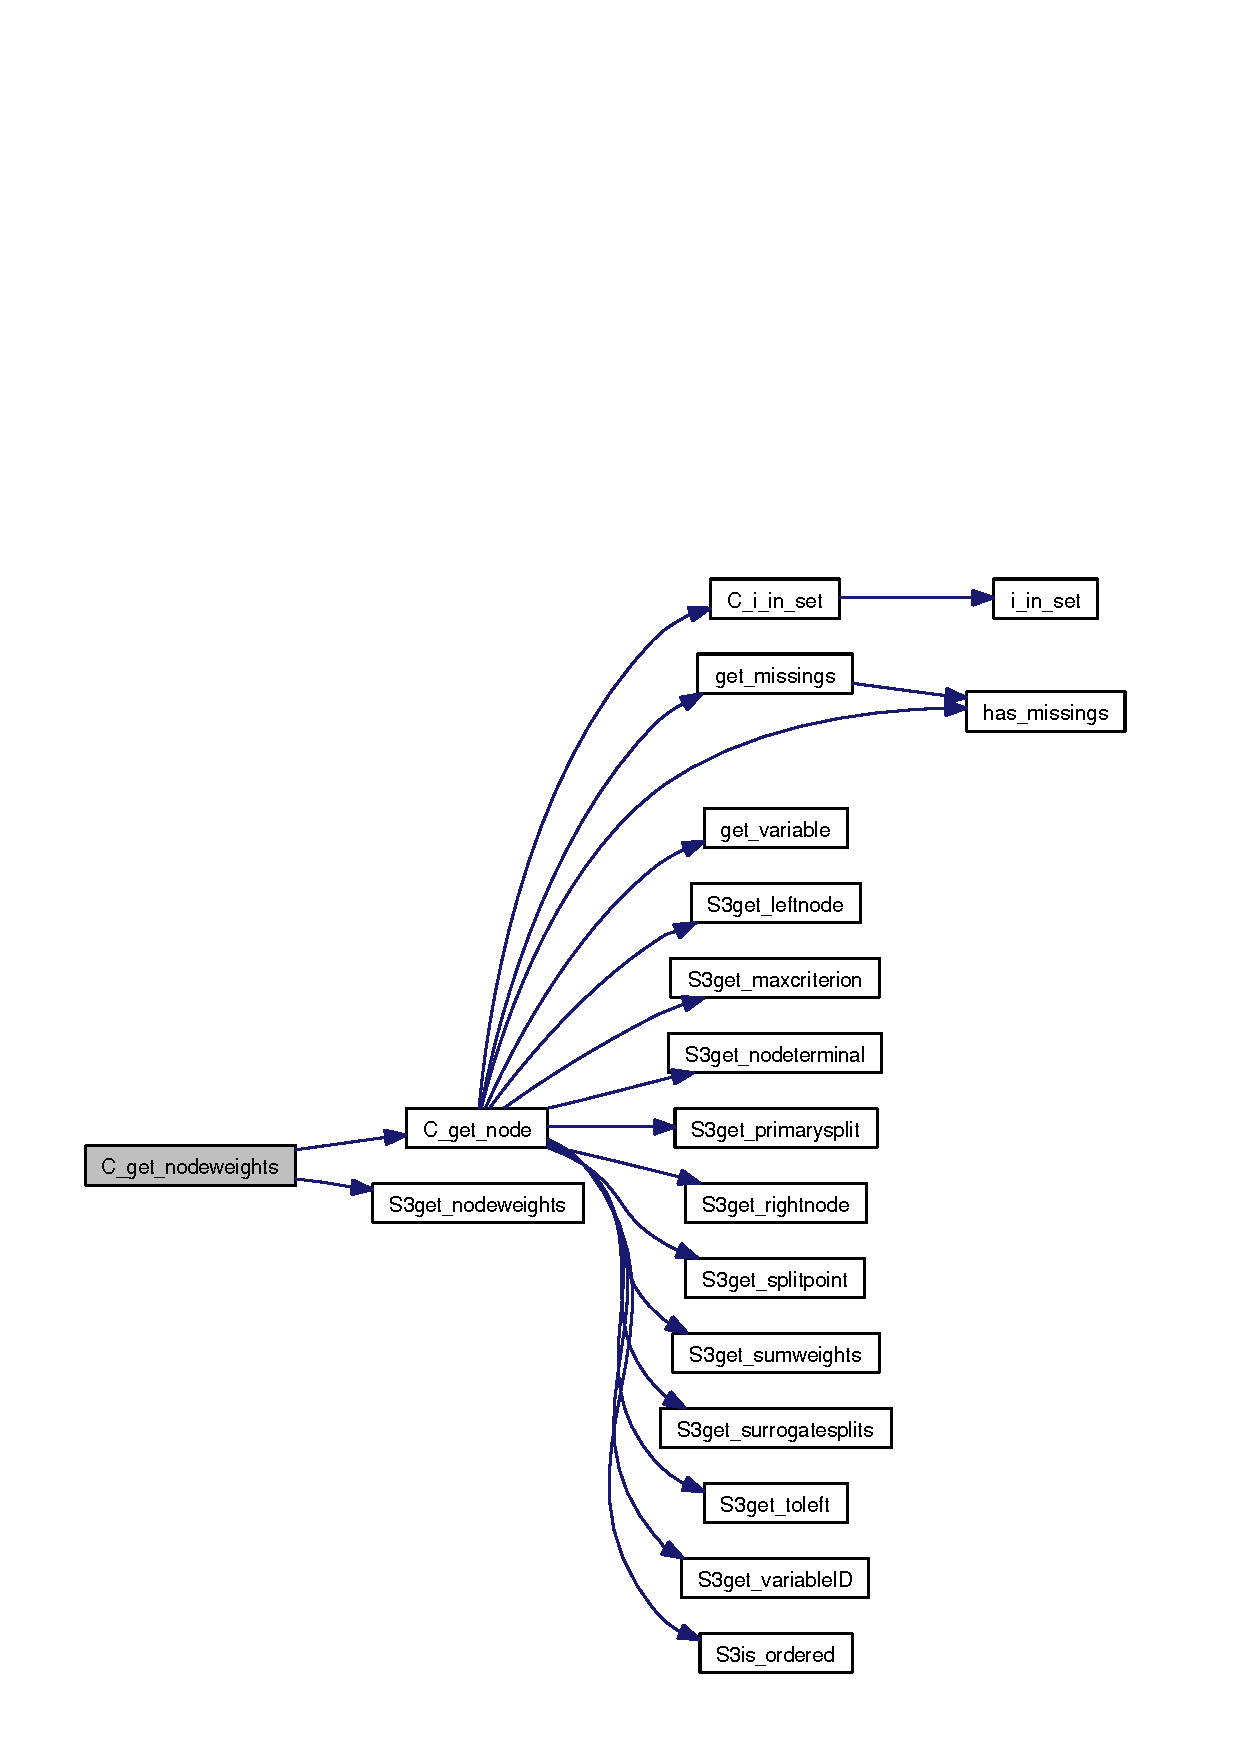
\includegraphics[width=257pt]{Predict_8c_cbb3e45d03e1b544c94bf639b191a953_cgraph}
\end{center}
\end{figure}
\hypertarget{Predict_8c_c4f4e806a78c376b13802ed2cf1e7b65}{
\index{Predict.c@{Predict.c}!C_get_prediction@{C\_\-get\_\-prediction}}
\index{C_get_prediction@{C\_\-get\_\-prediction}!Predict.c@{Predict.c}}
\subsubsection[C\_\-get\_\-prediction]{\setlength{\rightskip}{0pt plus 5cm}SEXP C\_\-get\_\-prediction (SEXP {\em subtree}, SEXP {\em newinputs}, double {\em mincriterion}, int {\em numobs})}}
\label{Predict_8c_c4f4e806a78c376b13802ed2cf1e7b65}


Get the prediction of a new observation\par
 \begin{Desc}
\item[Parameters:]
\begin{description}
\item[{\em subtree}]a tree \item[{\em newinputs}]an object of class `Variable\-Frame' \item[{\em mincriterion}]overwrites mincriterion used for tree growing \item[{\em numobs}]observation number \end{description}
\end{Desc}


Definition at line 284 of file Predict.c.

References C\_\-get\_\-node(), and S3get\_\-prediction().

Referenced by C\_\-predict().

Here is the call graph for this function:\begin{figure}[H]
\begin{center}
\leavevmode
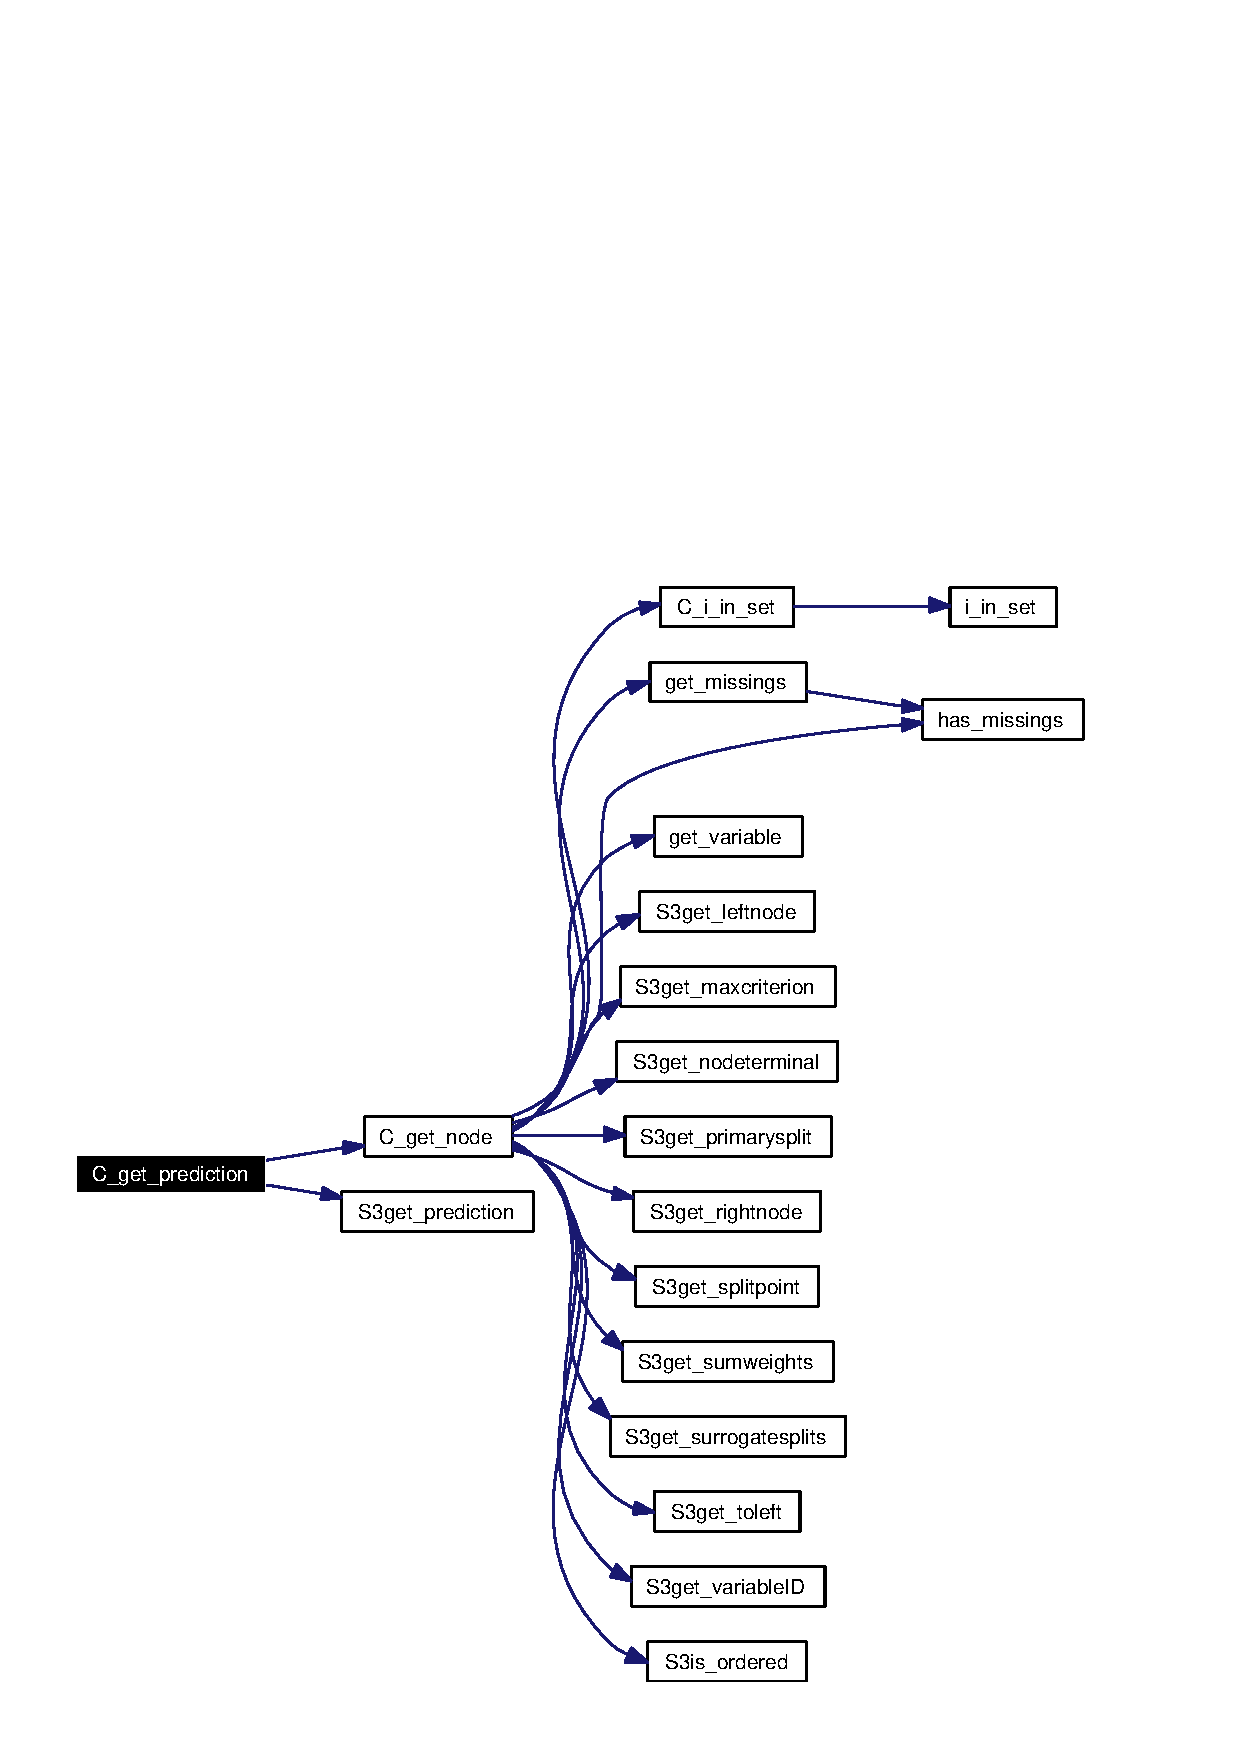
\includegraphics[width=260pt]{Predict_8c_c4f4e806a78c376b13802ed2cf1e7b65_cgraph}
\end{center}
\end{figure}
\hypertarget{Predict_8c_8964e7493ed9cb96c271b168b721e329}{
\index{Predict.c@{Predict.c}!C_getpredictions@{C\_\-getpredictions}}
\index{C_getpredictions@{C\_\-getpredictions}!Predict.c@{Predict.c}}
\subsubsection[C\_\-getpredictions]{\setlength{\rightskip}{0pt plus 5cm}void C\_\-getpredictions (SEXP {\em tree}, SEXP {\em where}, SEXP {\em ans})}}
\label{Predict_8c_8964e7493ed9cb96c271b168b721e329}


Get the predictions from `where' nodes\par
 \begin{Desc}
\item[Parameters:]
\begin{description}
\item[{\em tree}]a tree \item[{\em where}]vector of node\-ID's \item[{\em ans}]return value \end{description}
\end{Desc}


Definition at line 392 of file Predict.c.

References C\_\-get\_\-nodebynum(), and S3get\_\-prediction().

Referenced by R\_\-getpredictions().

Here is the call graph for this function:\begin{figure}[H]
\begin{center}
\leavevmode
\includegraphics[width=204pt]{Predict_8c_8964e7493ed9cb96c271b168b721e329_cgraph}
\end{center}
\end{figure}
\hypertarget{Predict_8c_1e3892117a14a178e707acf56ab56f5c}{
\index{Predict.c@{Predict.c}!C_getweights@{C\_\-getweights}}
\index{C_getweights@{C\_\-getweights}!Predict.c@{Predict.c}}
\subsubsection[C\_\-getweights]{\setlength{\rightskip}{0pt plus 5cm}void C\_\-getweights (SEXP {\em tree}, SEXP {\em where}, SEXP {\em ans})}}
\label{Predict_8c_1e3892117a14a178e707acf56ab56f5c}


Get the weights from `where' nodes\par
 \begin{Desc}
\item[Parameters:]
\begin{description}
\item[{\em tree}]a tree \item[{\em where}]vector of node\-ID's \item[{\em ans}]return value \end{description}
\end{Desc}


Definition at line 433 of file Predict.c.

References C\_\-get\_\-nodebynum(), and S3get\_\-nodeweights().

Referenced by R\_\-getweights().

Here is the call graph for this function:\begin{figure}[H]
\begin{center}
\leavevmode
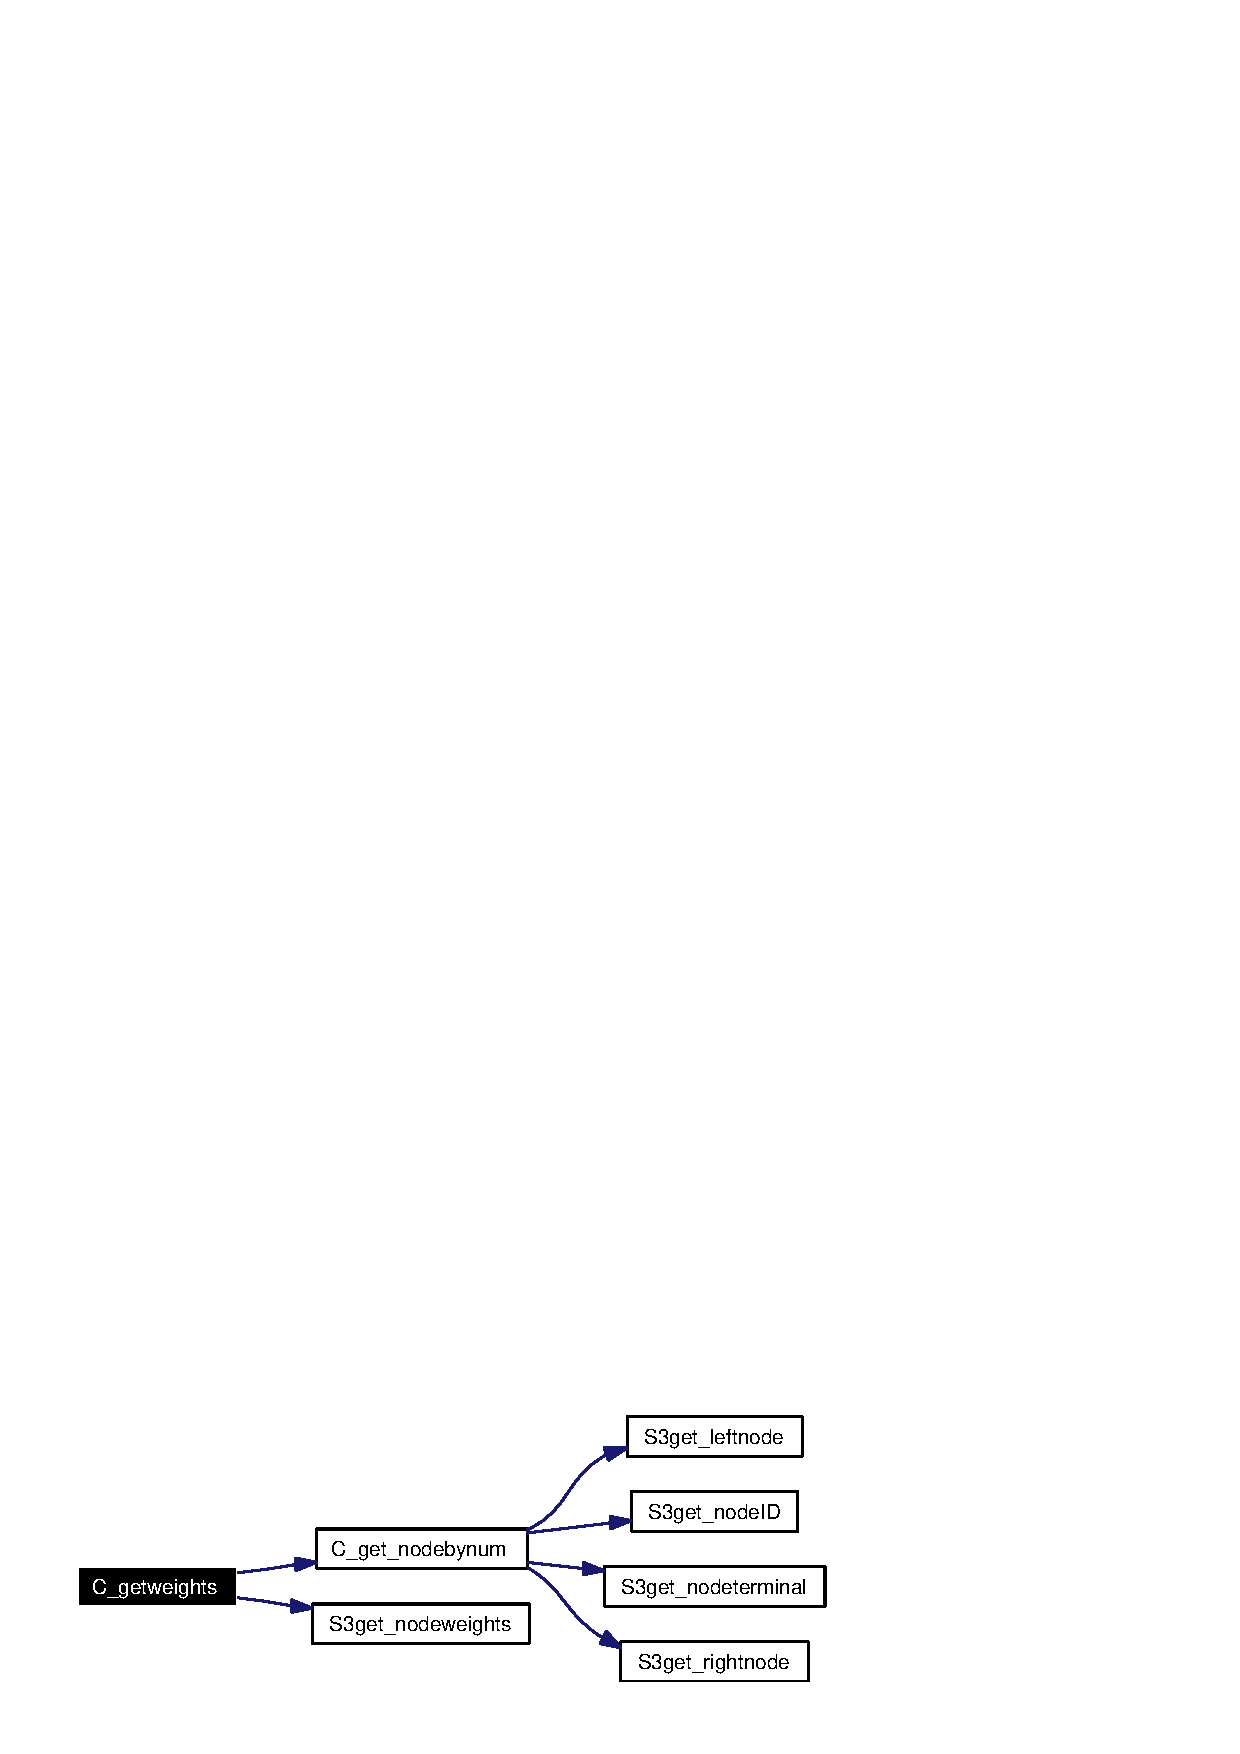
\includegraphics[width=198pt]{Predict_8c_1e3892117a14a178e707acf56ab56f5c_cgraph}
\end{center}
\end{figure}
\hypertarget{Predict_8c_ac36eff20575604b5d7558d512601d64}{
\index{Predict.c@{Predict.c}!C_predict@{C\_\-predict}}
\index{C_predict@{C\_\-predict}!Predict.c@{Predict.c}}
\subsubsection[C\_\-predict]{\setlength{\rightskip}{0pt plus 5cm}void C\_\-predict (SEXP {\em tree}, SEXP {\em newinputs}, double {\em mincriterion}, SEXP {\em ans})}}
\label{Predict_8c_ac36eff20575604b5d7558d512601d64}


Get all predictions for `newinputs' \par
 \begin{Desc}
\item[Parameters:]
\begin{description}
\item[{\em tree}]a tree \item[{\em newinputs}]an object of class `Variable\-Frame' \item[{\em mincriterion}]overwrites mincriterion used for tree growing \item[{\em ans}]return value \end{description}
\end{Desc}


Definition at line 351 of file Predict.c.

References C\_\-get\_\-prediction(), and get\_\-nobs().

Referenced by R\_\-predict().

Here is the call graph for this function:\begin{figure}[H]
\begin{center}
\leavevmode
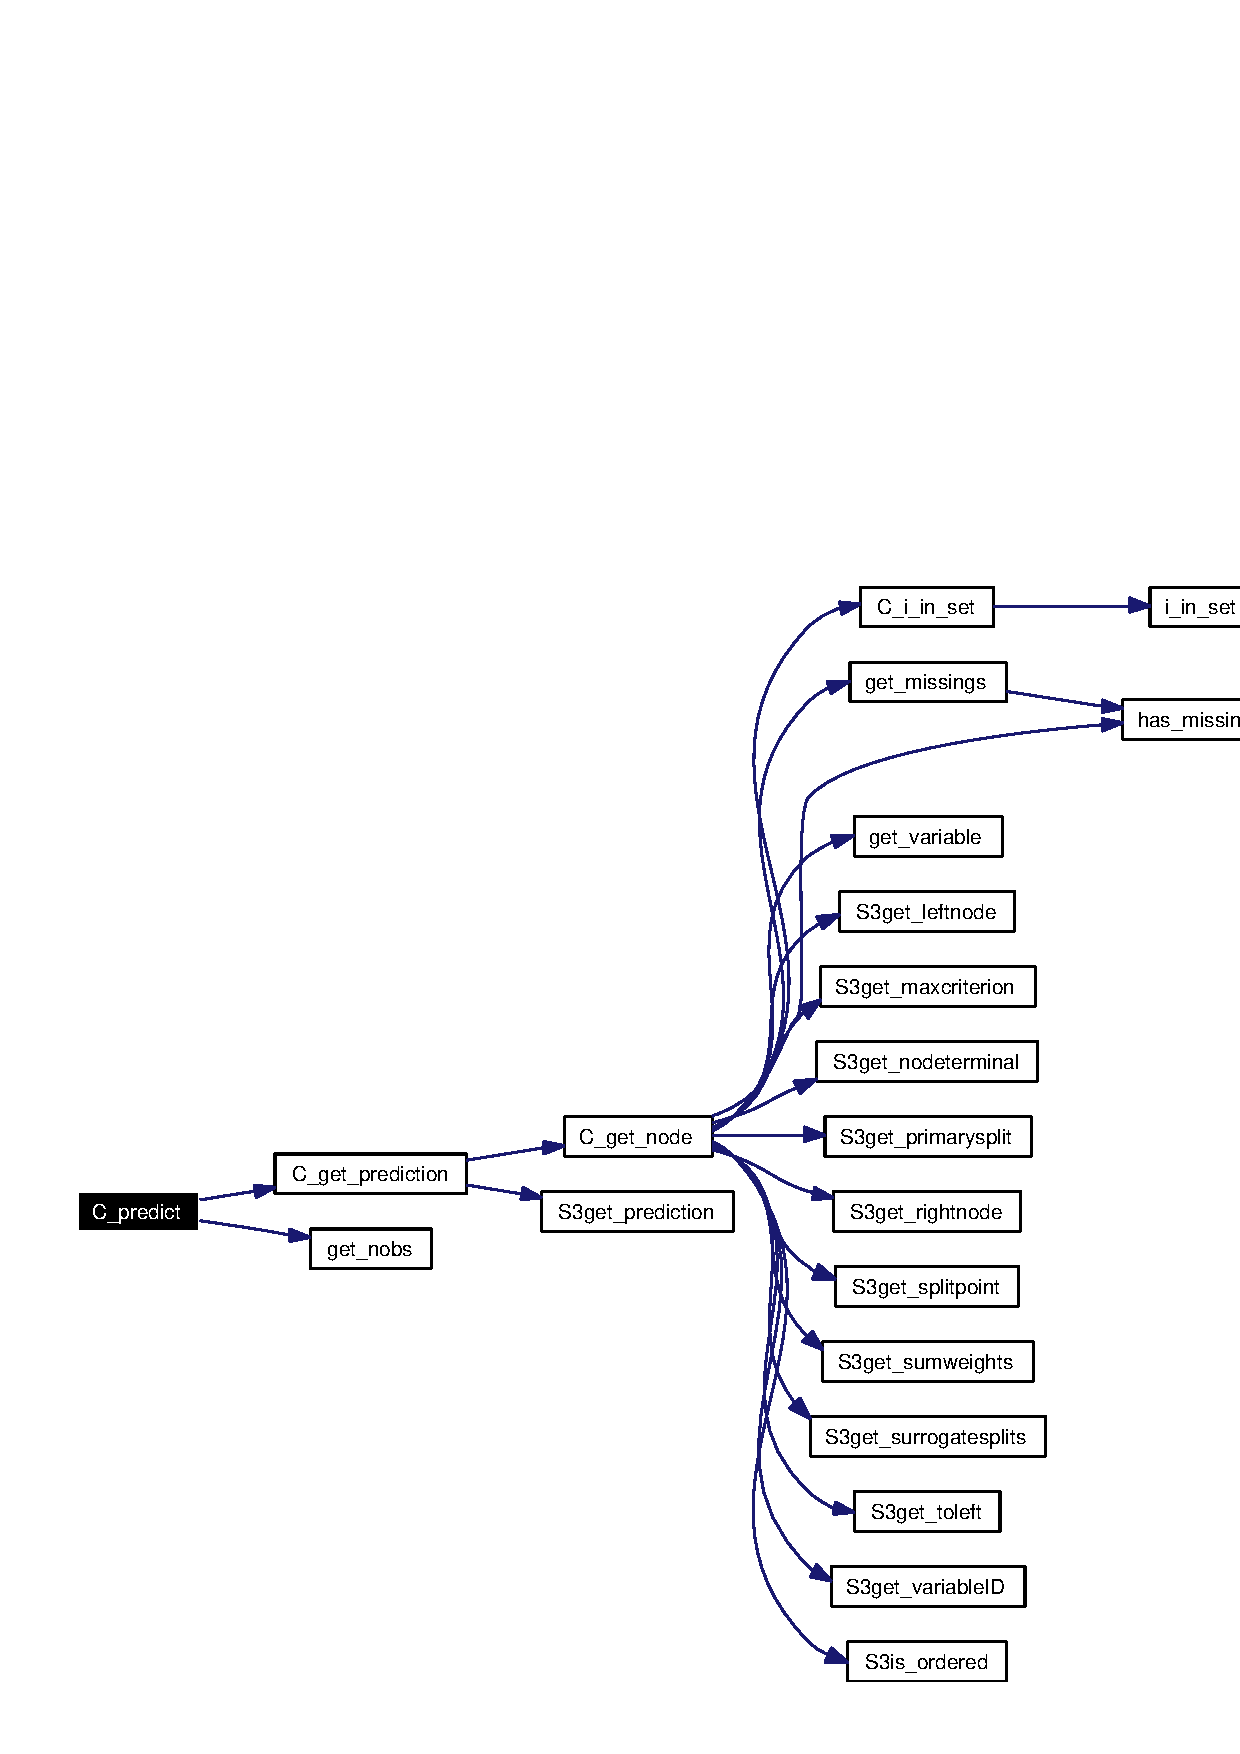
\includegraphics[width=308pt]{Predict_8c_ac36eff20575604b5d7558d512601d64_cgraph}
\end{center}
\end{figure}
\hypertarget{Predict_8c_daf8a0eb8790ebf14f0e265de164d50e}{
\index{Predict.c@{Predict.c}!C_splitnode@{C\_\-splitnode}}
\index{C_splitnode@{C\_\-splitnode}!Predict.c@{Predict.c}}
\subsubsection[C\_\-splitnode]{\setlength{\rightskip}{0pt plus 5cm}void C\_\-splitnode (SEXP {\em node}, SEXP {\em learnsample}, SEXP {\em control})}}
\label{Predict_8c_daf8a0eb8790ebf14f0e265de164d50e}


Split a node according to a splitting rule \par
 \begin{Desc}
\item[Parameters:]
\begin{description}
\item[{\em node}]the current node with primary split specified \item[{\em learnsample}]learning sample \item[{\em control}]an object of class `Tree\-Control' \end{description}
\end{Desc}
\begin{Desc}
\item[\hyperlink{todo__todo000001}{Todo}]outplace the splitting since there are at least 3 functions with nearly identical code \end{Desc}


Definition at line 21 of file Predict.c.

References C\_\-init\_\-node(), get\_\-maxsurrogate(), get\_\-missings(), get\_\-ninputs(), get\_\-nobs(), get\_\-predict\_\-trafo(), get\_\-splitctrl(), get\_\-variable(), has\_\-missings(), i\_\-in\_\-set(), ncol(), NODE\_\-LENGTH, PL2\_\-inputs\-Sym, PL2\_\-responses\-Sym, S3\_\-LEFT, S3\_\-RIGHT, S3get\_\-nodeweights(), S3get\_\-primarysplit(), S3get\_\-splitpoint(), S3get\_\-variable\-ID(), and S3is\_\-ordered().

Referenced by C\_\-Tree\-Grow().

Here is the call graph for this function:\begin{figure}[H]
\begin{center}
\leavevmode
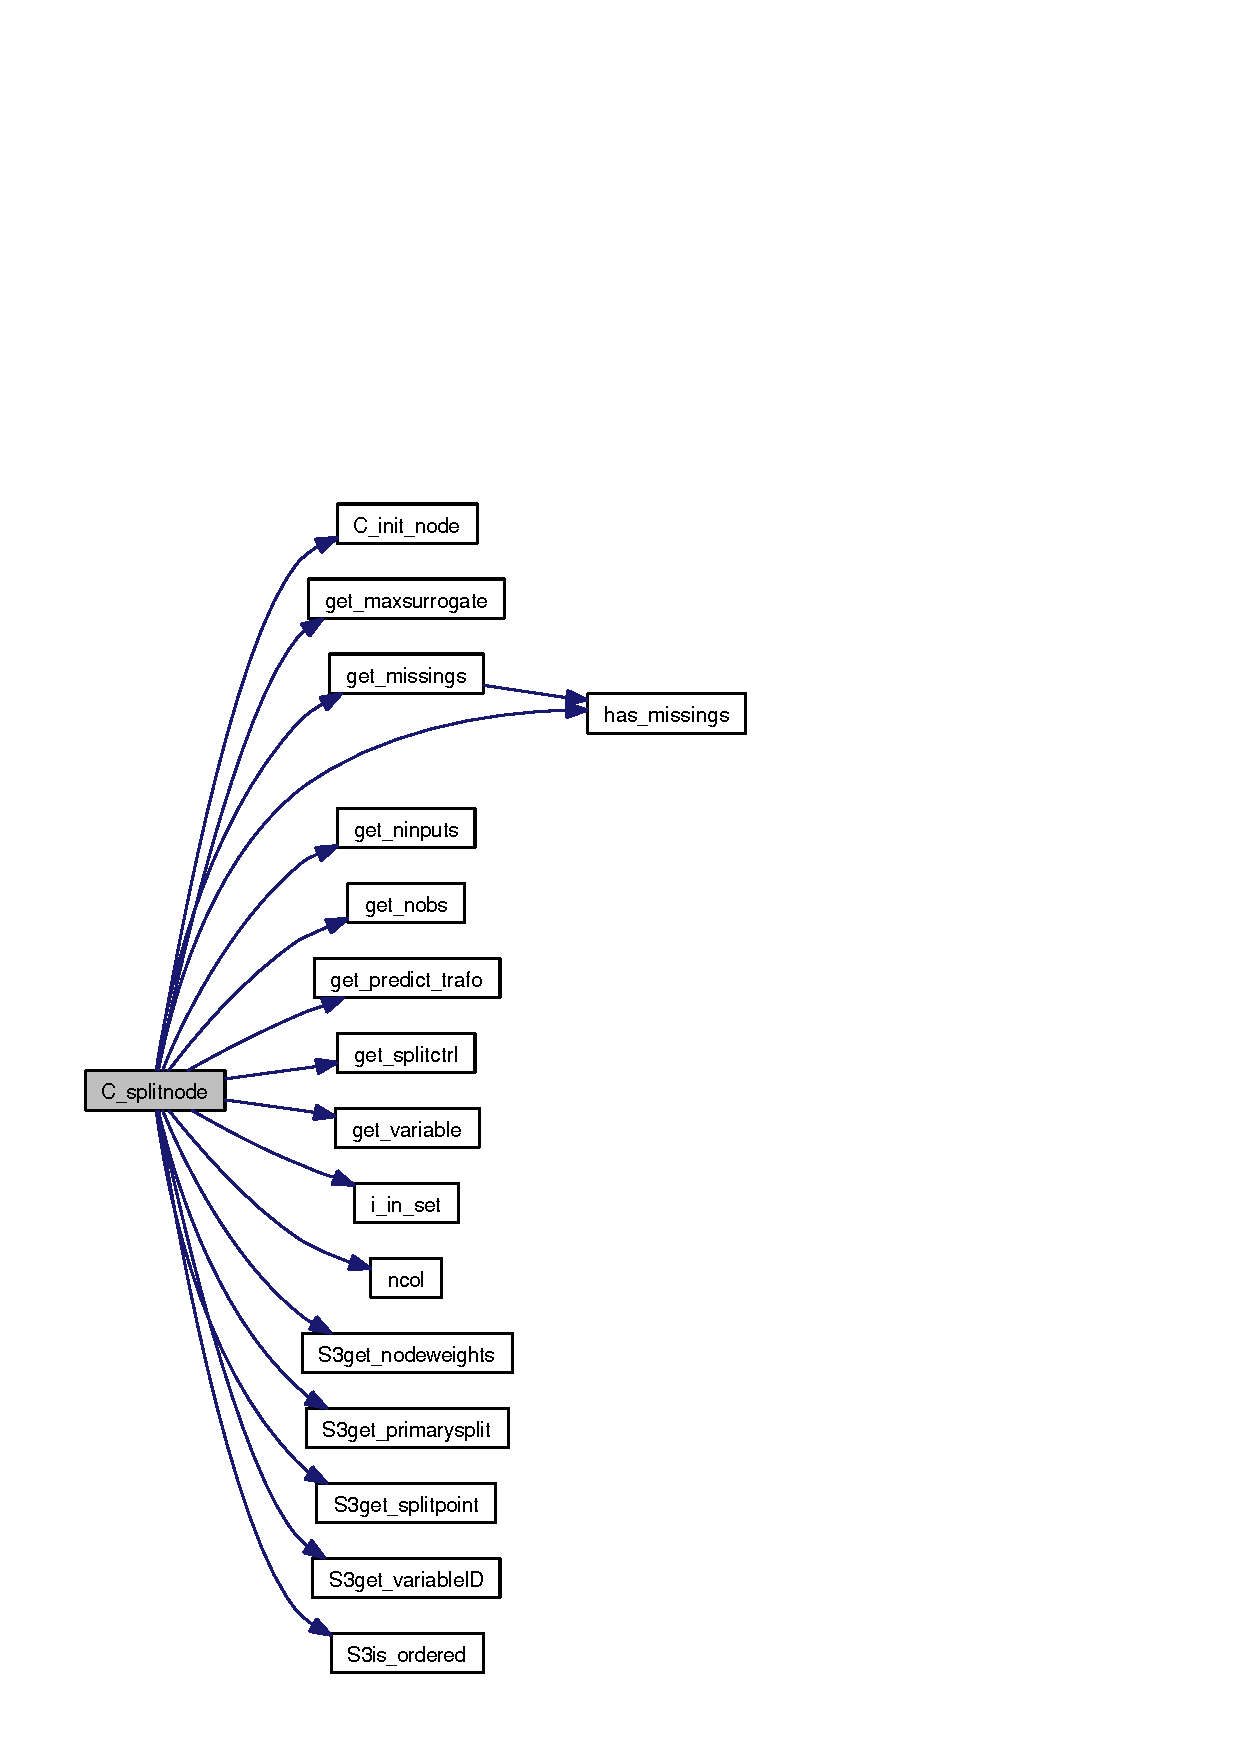
\includegraphics[width=180pt]{Predict_8c_daf8a0eb8790ebf14f0e265de164d50e_cgraph}
\end{center}
\end{figure}
\hypertarget{Predict_8c_830785cf09ef008b28bd8577feb6d06b}{
\index{Predict.c@{Predict.c}!C_weights@{C\_\-weights}}
\index{C_weights@{C\_\-weights}!Predict.c@{Predict.c}}
\subsubsection[C\_\-weights]{\setlength{\rightskip}{0pt plus 5cm}void C\_\-weights (SEXP {\em tree}, SEXP {\em newinputs}, double {\em mincriterion}, SEXP {\em ans})}}
\label{Predict_8c_830785cf09ef008b28bd8577feb6d06b}


Get the weights for all observations in `newinputs' \begin{Desc}
\item[Parameters:]
\begin{description}
\item[{\em tree}]a tree \item[{\em newinputs}]an object of class `Variable\-Frame' \item[{\em mincriterion}]overwrites mincriterion used for tree growing \item[{\em ans}]return value \end{description}
\end{Desc}


Definition at line 475 of file Predict.c.

References C\_\-get\_\-nodeweights(), and get\_\-nobs().

Referenced by R\_\-weights().

Here is the call graph for this function:\begin{figure}[H]
\begin{center}
\leavevmode
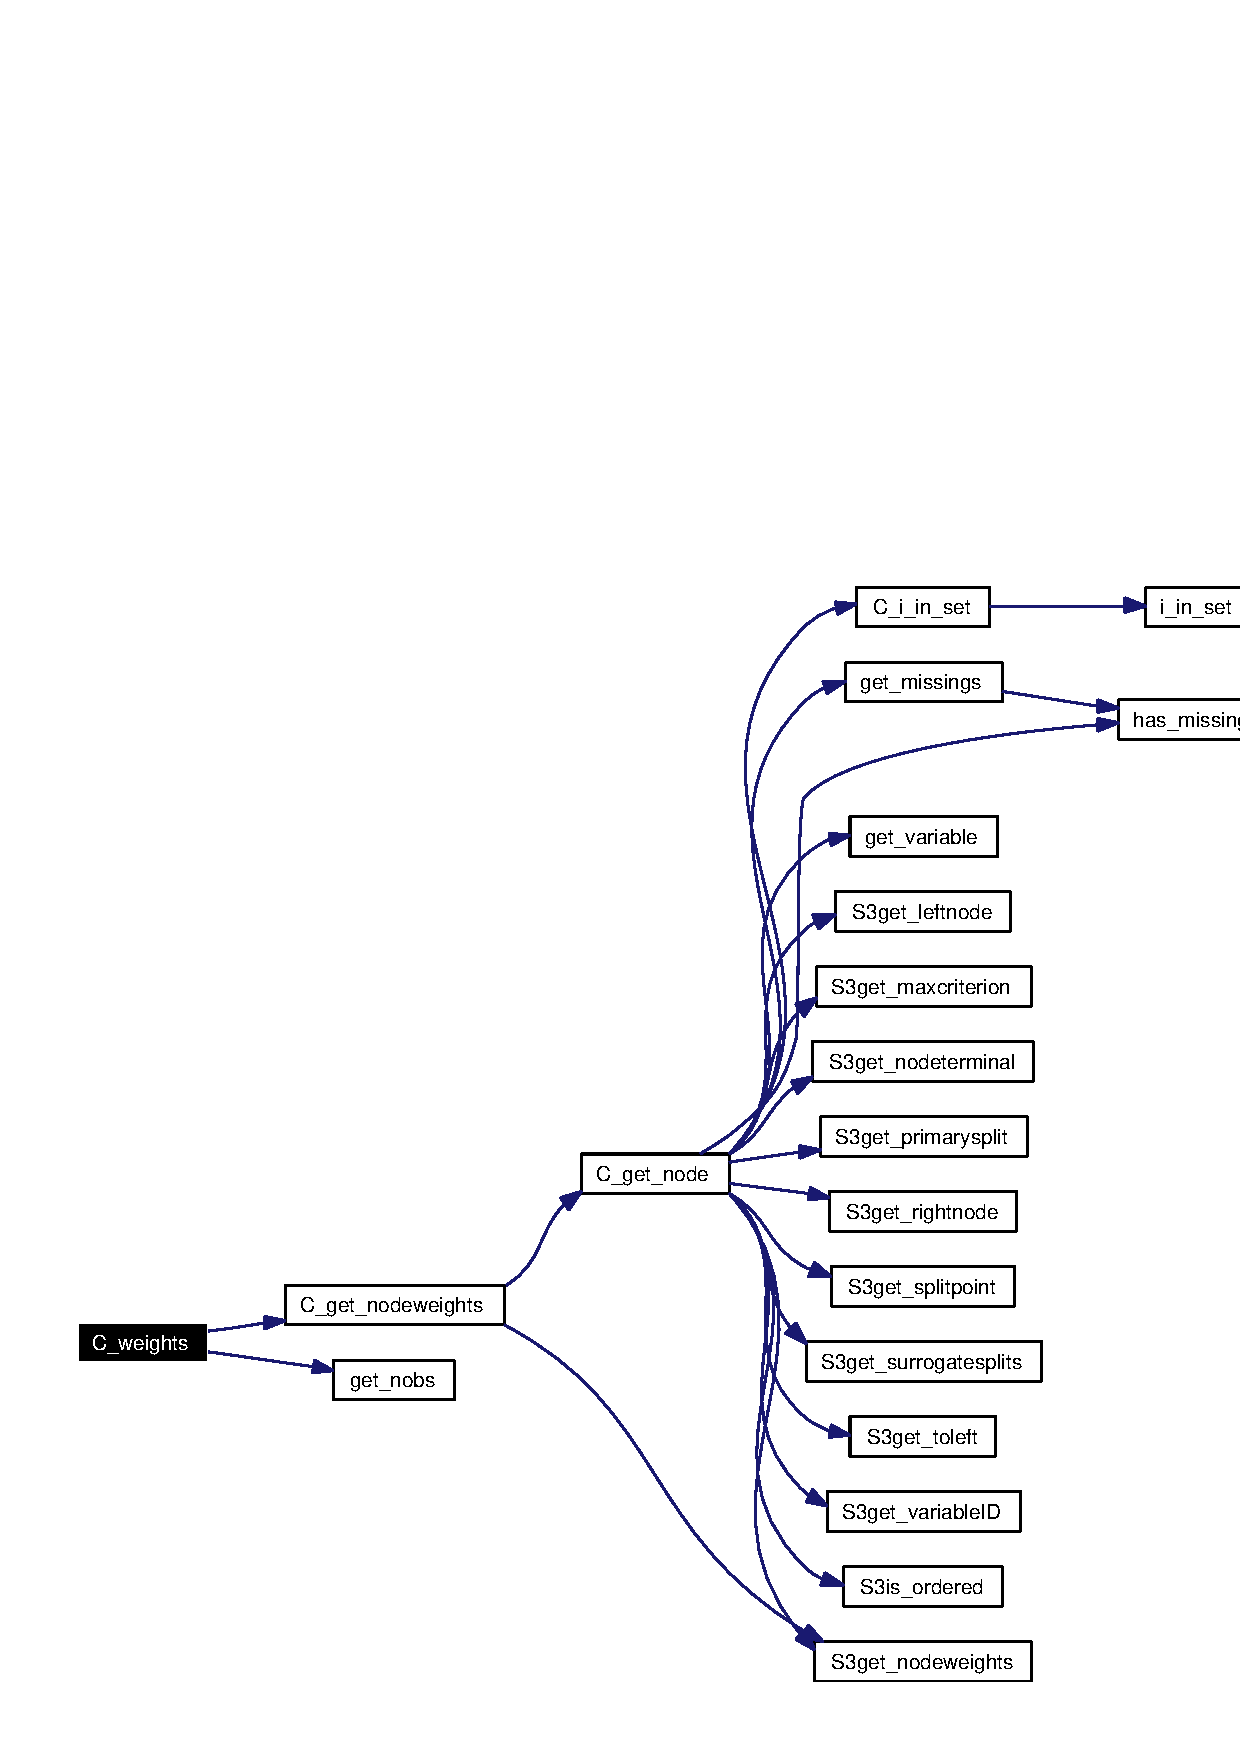
\includegraphics[width=307pt]{Predict_8c_830785cf09ef008b28bd8577feb6d06b_cgraph}
\end{center}
\end{figure}
\hypertarget{Predict_8c_dec31e3aa985e0af16ccaeac31237640}{
\index{Predict.c@{Predict.c}!R_get_node@{R\_\-get\_\-node}}
\index{R_get_node@{R\_\-get\_\-node}!Predict.c@{Predict.c}}
\subsubsection[R\_\-get\_\-node]{\setlength{\rightskip}{0pt plus 5cm}SEXP R\_\-get\_\-node (SEXP {\em subtree}, SEXP {\em newinputs}, SEXP {\em mincriterion}, SEXP {\em numobs})}}
\label{Predict_8c_dec31e3aa985e0af16ccaeac31237640}


R-Interface to C\_\-get\_\-node \par
 \begin{Desc}
\item[Parameters:]
\begin{description}
\item[{\em subtree}]a tree \item[{\em newinputs}]an object of class `Variable\-Frame' \item[{\em mincriterion}]overwrites mincriterion used for tree growing \item[{\em numobs}]observation number \end{description}
\end{Desc}


Definition at line 237 of file Predict.c.

References C\_\-get\_\-node().

Here is the call graph for this function:\begin{figure}[H]
\begin{center}
\leavevmode
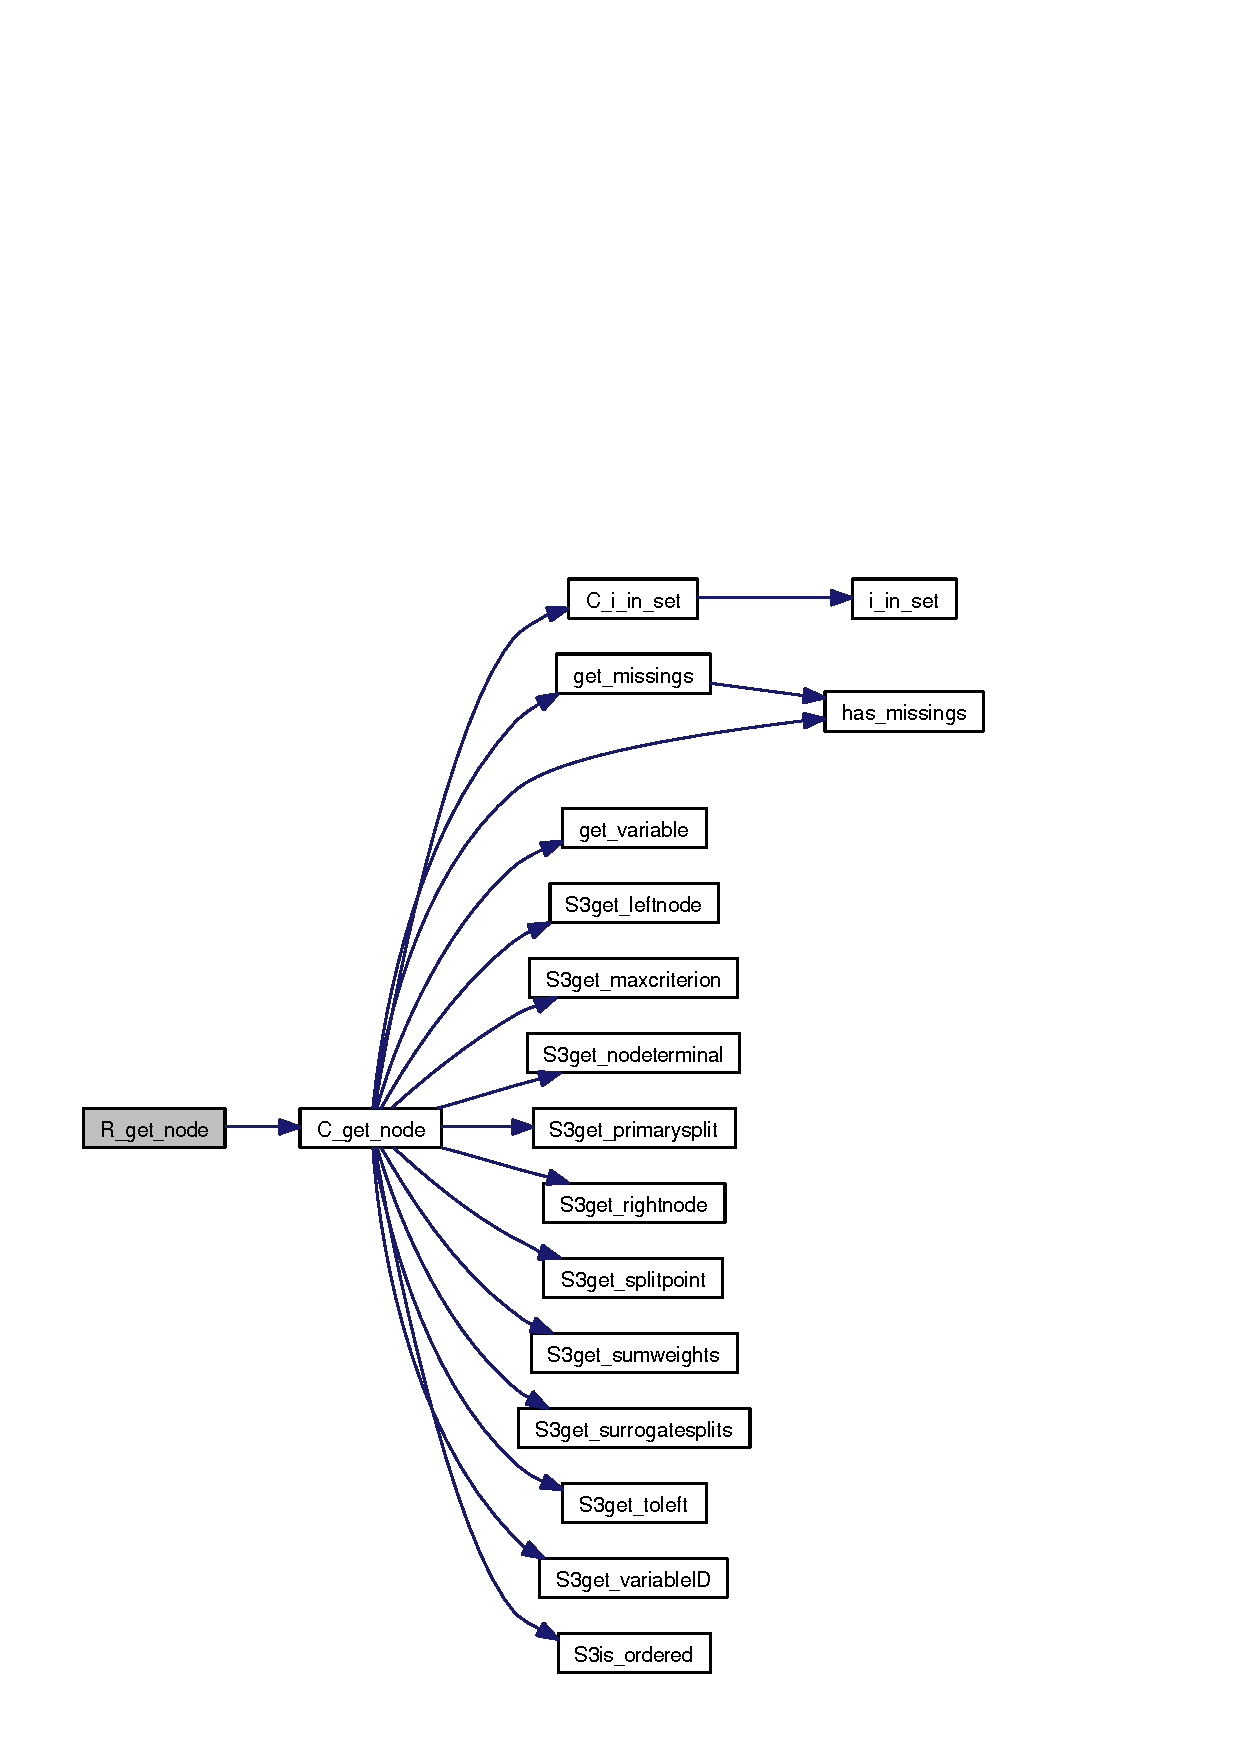
\includegraphics[width=240pt]{Predict_8c_dec31e3aa985e0af16ccaeac31237640_cgraph}
\end{center}
\end{figure}
\hypertarget{Predict_8c_4a30a8aa916f294059b6e2cbcb9e29d5}{
\index{Predict.c@{Predict.c}!R_get_nodebynum@{R\_\-get\_\-nodebynum}}
\index{R_get_nodebynum@{R\_\-get\_\-nodebynum}!Predict.c@{Predict.c}}
\subsubsection[R\_\-get\_\-nodebynum]{\setlength{\rightskip}{0pt plus 5cm}SEXP R\_\-get\_\-nodebynum (SEXP {\em subtree}, SEXP {\em nodenum})}}
\label{Predict_8c_4a30a8aa916f294059b6e2cbcb9e29d5}


R-Interface to C\_\-get\_\-nodenum \par
 \begin{Desc}
\item[Parameters:]
\begin{description}
\item[{\em subtree}]a tree \item[{\em nodenum}]a node\-ID \end{description}
\end{Desc}


Definition at line 271 of file Predict.c.

References C\_\-get\_\-nodebynum().

Here is the call graph for this function:\begin{figure}[H]
\begin{center}
\leavevmode
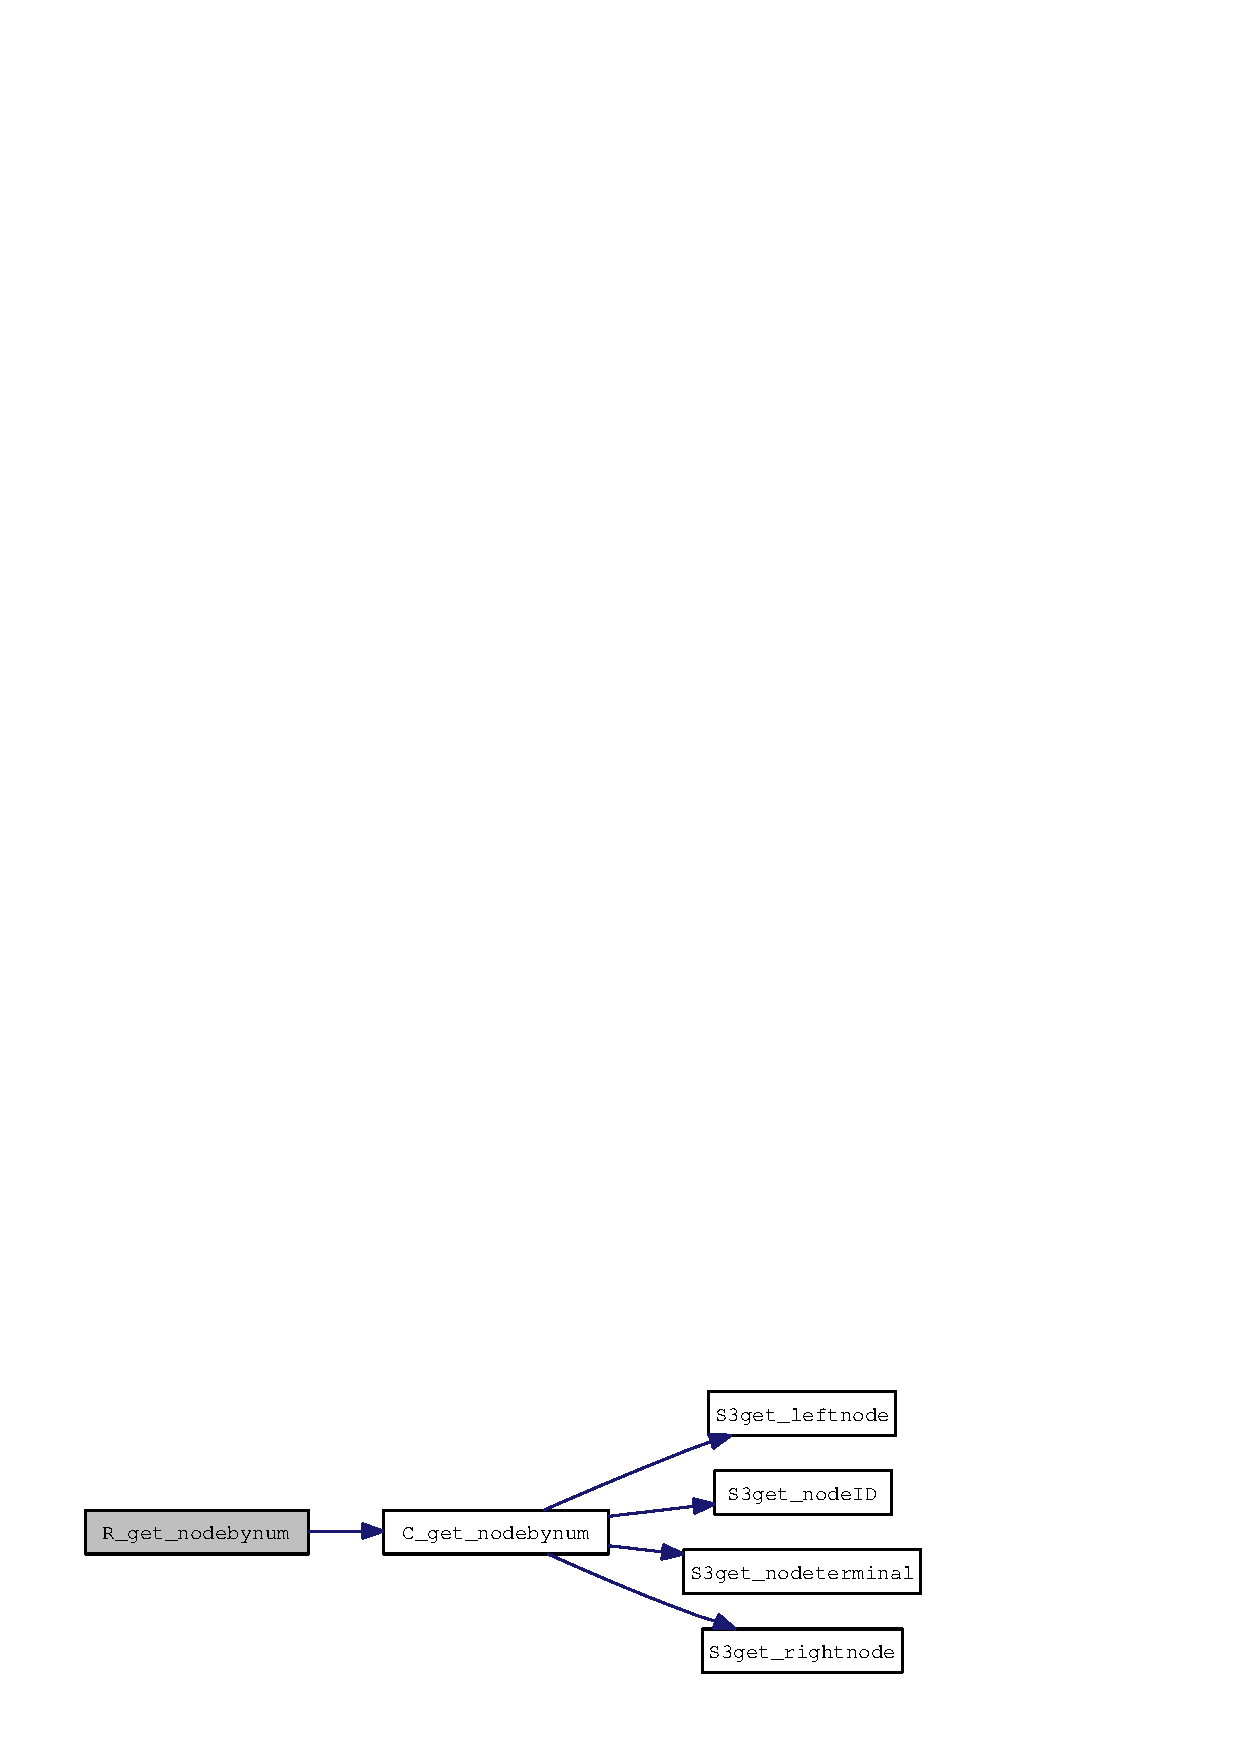
\includegraphics[width=209pt]{Predict_8c_4a30a8aa916f294059b6e2cbcb9e29d5_cgraph}
\end{center}
\end{figure}
\hypertarget{Predict_8c_c0668d268fe5a4bad29fbf4ead39c526}{
\index{Predict.c@{Predict.c}!R_get_nodeID@{R\_\-get\_\-nodeID}}
\index{R_get_nodeID@{R\_\-get\_\-nodeID}!Predict.c@{Predict.c}}
\subsubsection[R\_\-get\_\-nodeID]{\setlength{\rightskip}{0pt plus 5cm}SEXP R\_\-get\_\-node\-ID (SEXP {\em tree}, SEXP {\em newinputs}, SEXP {\em mincriterion})}}
\label{Predict_8c_c0668d268fe5a4bad29fbf4ead39c526}


R-Interface to C\_\-get\_\-node\-ID \par
 \begin{Desc}
\item[Parameters:]
\begin{description}
\item[{\em tree}]a tree \item[{\em newinputs}]an object of class `Variable\-Frame' \item[{\em mincriterion}]overwrites mincriterion used for tree growing \end{description}
\end{Desc}


Definition at line 328 of file Predict.c.

References C\_\-get\_\-node\-ID(), and get\_\-nobs().

Here is the call graph for this function:\begin{figure}[H]
\begin{center}
\leavevmode
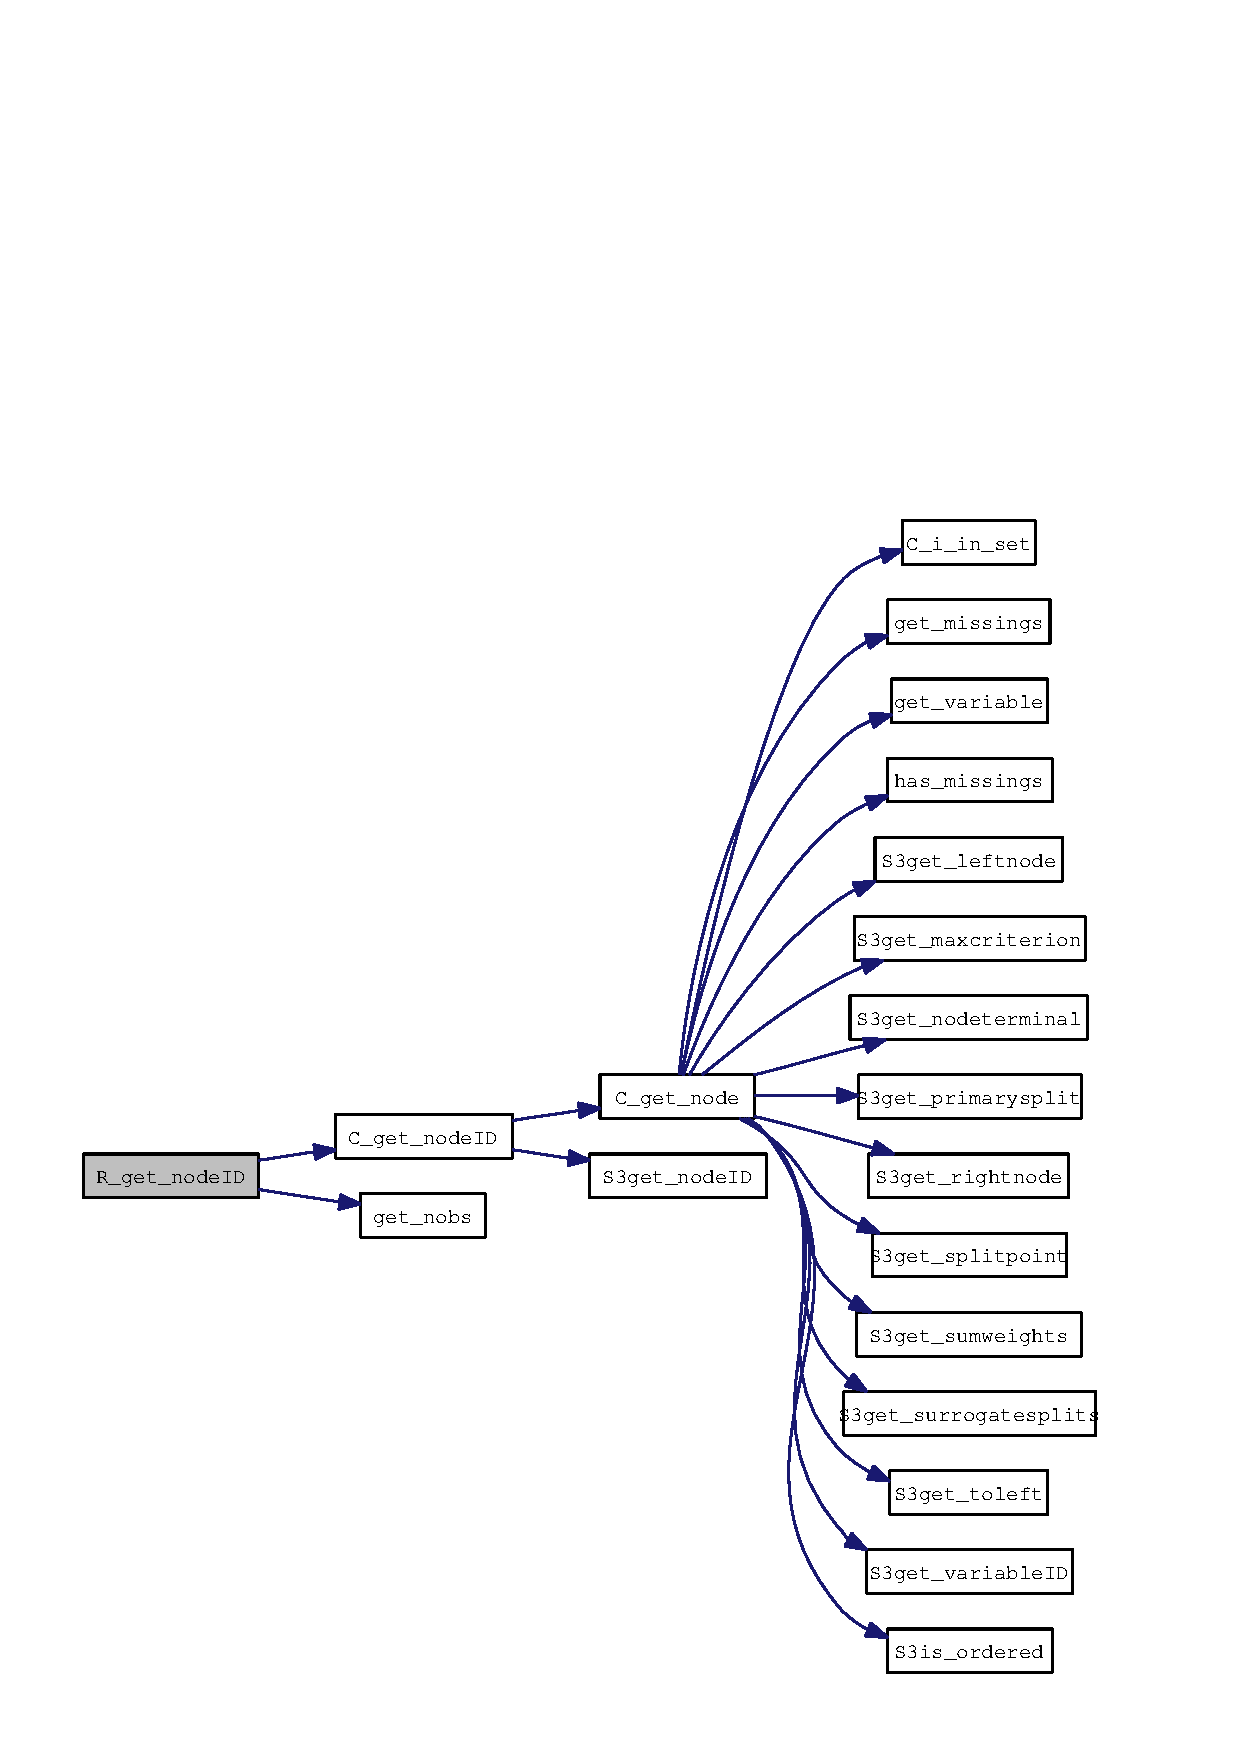
\includegraphics[width=308pt]{Predict_8c_c0668d268fe5a4bad29fbf4ead39c526_cgraph}
\end{center}
\end{figure}
\hypertarget{Predict_8c_a508a31f1fd7cd3668ad81eb0d00dd66}{
\index{Predict.c@{Predict.c}!R_getpredictions@{R\_\-getpredictions}}
\index{R_getpredictions@{R\_\-getpredictions}!Predict.c@{Predict.c}}
\subsubsection[R\_\-getpredictions]{\setlength{\rightskip}{0pt plus 5cm}SEXP R\_\-getpredictions (SEXP {\em tree}, SEXP {\em where})}}
\label{Predict_8c_a508a31f1fd7cd3668ad81eb0d00dd66}


R-Interface to C\_\-getpredictions\par
 \begin{Desc}
\item[Parameters:]
\begin{description}
\item[{\em tree}]a tree \item[{\em where}]vector of node\-ID's \end{description}
\end{Desc}


Definition at line 413 of file Predict.c.

References C\_\-getpredictions().

Here is the call graph for this function:\begin{figure}[H]
\begin{center}
\leavevmode
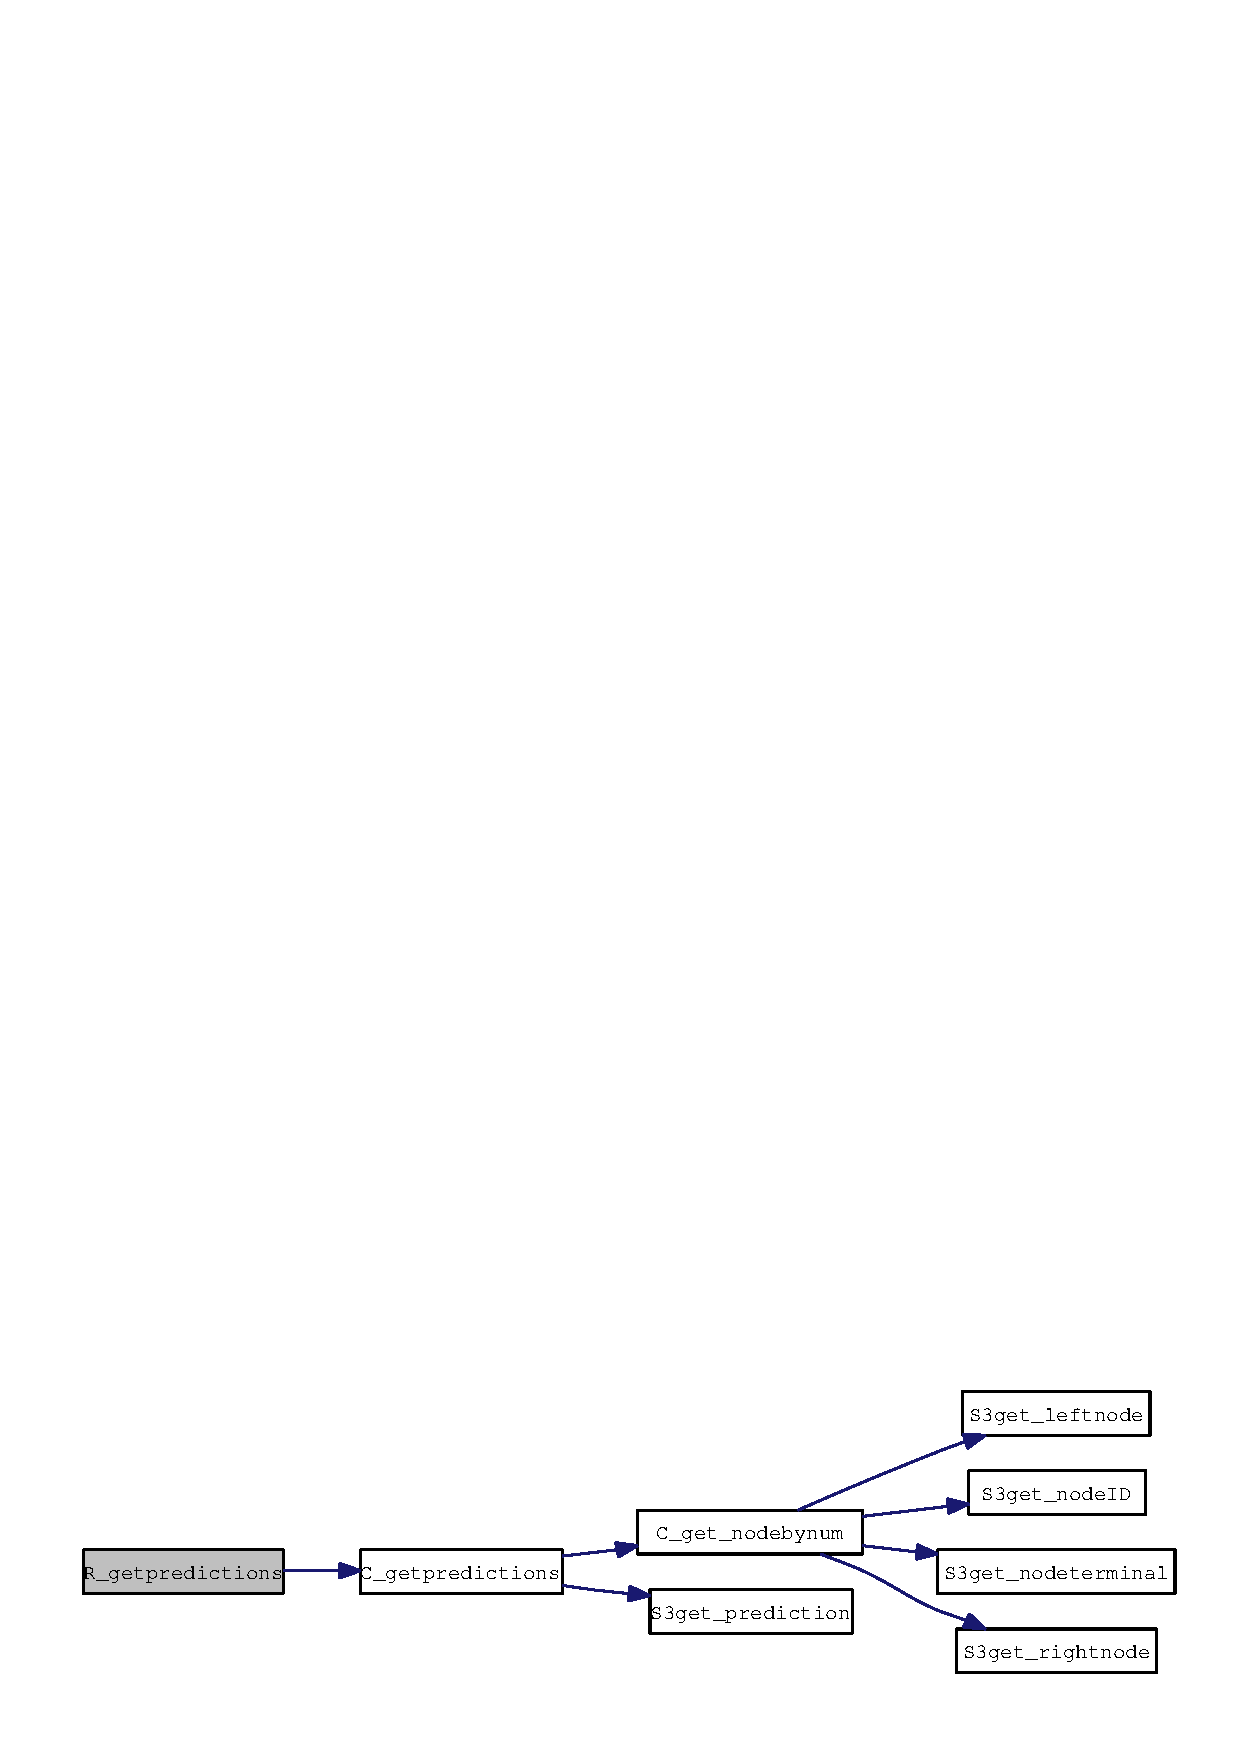
\includegraphics[width=268pt]{Predict_8c_a508a31f1fd7cd3668ad81eb0d00dd66_cgraph}
\end{center}
\end{figure}
\hypertarget{Predict_8c_f255340d550e1387709b1674467c31b9}{
\index{Predict.c@{Predict.c}!R_getweights@{R\_\-getweights}}
\index{R_getweights@{R\_\-getweights}!Predict.c@{Predict.c}}
\subsubsection[R\_\-getweights]{\setlength{\rightskip}{0pt plus 5cm}SEXP R\_\-getweights (SEXP {\em tree}, SEXP {\em where})}}
\label{Predict_8c_f255340d550e1387709b1674467c31b9}


R-Interface to C\_\-getweigts \par
 \begin{Desc}
\item[Parameters:]
\begin{description}
\item[{\em tree}]a tree \item[{\em where}]vector of node\-ID's \end{description}
\end{Desc}


Definition at line 454 of file Predict.c.

References C\_\-getweights().

Here is the call graph for this function:\begin{figure}[H]
\begin{center}
\leavevmode
\includegraphics[width=255pt]{Predict_8c_f255340d550e1387709b1674467c31b9_cgraph}
\end{center}
\end{figure}
\hypertarget{Predict_8c_9a5170a24bc00b727527b80cec5ca60a}{
\index{Predict.c@{Predict.c}!R_predict@{R\_\-predict}}
\index{R_predict@{R\_\-predict}!Predict.c@{Predict.c}}
\subsubsection[R\_\-predict]{\setlength{\rightskip}{0pt plus 5cm}SEXP R\_\-predict (SEXP {\em tree}, SEXP {\em newinputs}, SEXP {\em mincriterion})}}
\label{Predict_8c_9a5170a24bc00b727527b80cec5ca60a}


R-Interface to C\_\-predict \par
 \begin{Desc}
\item[Parameters:]
\begin{description}
\item[{\em tree}]a tree \item[{\em newinputs}]an object of class `Variable\-Frame' \item[{\em mincriterion}]overwrites mincriterion used for tree growing \end{description}
\end{Desc}


Definition at line 372 of file Predict.c.

References C\_\-predict(), and get\_\-nobs().

Here is the call graph for this function:\begin{figure}[H]
\begin{center}
\leavevmode
\includegraphics[width=356pt]{Predict_8c_9a5170a24bc00b727527b80cec5ca60a_cgraph}
\end{center}
\end{figure}
\hypertarget{Predict_8c_20dd01c361767edbfc62abf55ce30ff1}{
\index{Predict.c@{Predict.c}!R_predictRF@{R\_\-predictRF}}
\index{R_predictRF@{R\_\-predictRF}!Predict.c@{Predict.c}}
\subsubsection[R\_\-predictRF]{\setlength{\rightskip}{0pt plus 5cm}SEXP R\_\-predict\-RF (SEXP {\em forest}, SEXP {\em newinputs}, SEXP {\em mincriterion}, SEXP {\em oobpred})}}
\label{Predict_8c_20dd01c361767edbfc62abf55ce30ff1}


Predictions from Random\-Forest objects \begin{Desc}
\item[Parameters:]
\begin{description}
\item[{\em forest}]a list of trees \item[{\em newinputs}]an object of class `Variable\-Frame' \item[{\em mincriterion}]overwrites mincriterion used for tree growing \item[{\em oobpred}]a logical indicating out-of-bag predictions \end{description}
\end{Desc}


Definition at line 518 of file Predict.c.

References C\_\-get\_\-nodebynum(), C\_\-get\_\-node\-ID(), get\_\-nobs(), S3get\_\-nodeweights(), and S3get\_\-prediction().

Here is the call graph for this function:\begin{figure}[H]
\begin{center}
\leavevmode
\includegraphics[width=320pt]{Predict_8c_20dd01c361767edbfc62abf55ce30ff1_cgraph}
\end{center}
\end{figure}
\hypertarget{Predict_8c_a4f23088af5379408f00d3809656d0da}{
\index{Predict.c@{Predict.c}!R_predictRF2@{R\_\-predictRF2}}
\index{R_predictRF2@{R\_\-predictRF2}!Predict.c@{Predict.c}}
\subsubsection[R\_\-predictRF2]{\setlength{\rightskip}{0pt plus 5cm}SEXP R\_\-predict\-RF2 (SEXP {\em forest}, SEXP {\em response}, SEXP {\em newinputs}, SEXP {\em mincriterion}, SEXP {\em oobpred})}}
\label{Predict_8c_a4f23088af5379408f00d3809656d0da}


Predictions from Random\-Forest objects, based in total weights \begin{Desc}
\item[Parameters:]
\begin{description}
\item[{\em forest}]a list of trees \item[{\em response}]a matrix of (transformed) response values \item[{\em newinputs}]an object of class `Variable\-Frame' \item[{\em mincriterion}]overwrites mincriterion used for tree growing \item[{\em oobpred}]a logical indicating out-of-bag predictions \end{description}
\end{Desc}


Definition at line 574 of file Predict.c.

References C\_\-get\_\-nodebynum(), C\_\-get\_\-node\-ID(), get\_\-nobs(), ncol(), nrow(), and S3get\_\-nodeweights().

Here is the call graph for this function:\begin{figure}[H]
\begin{center}
\leavevmode
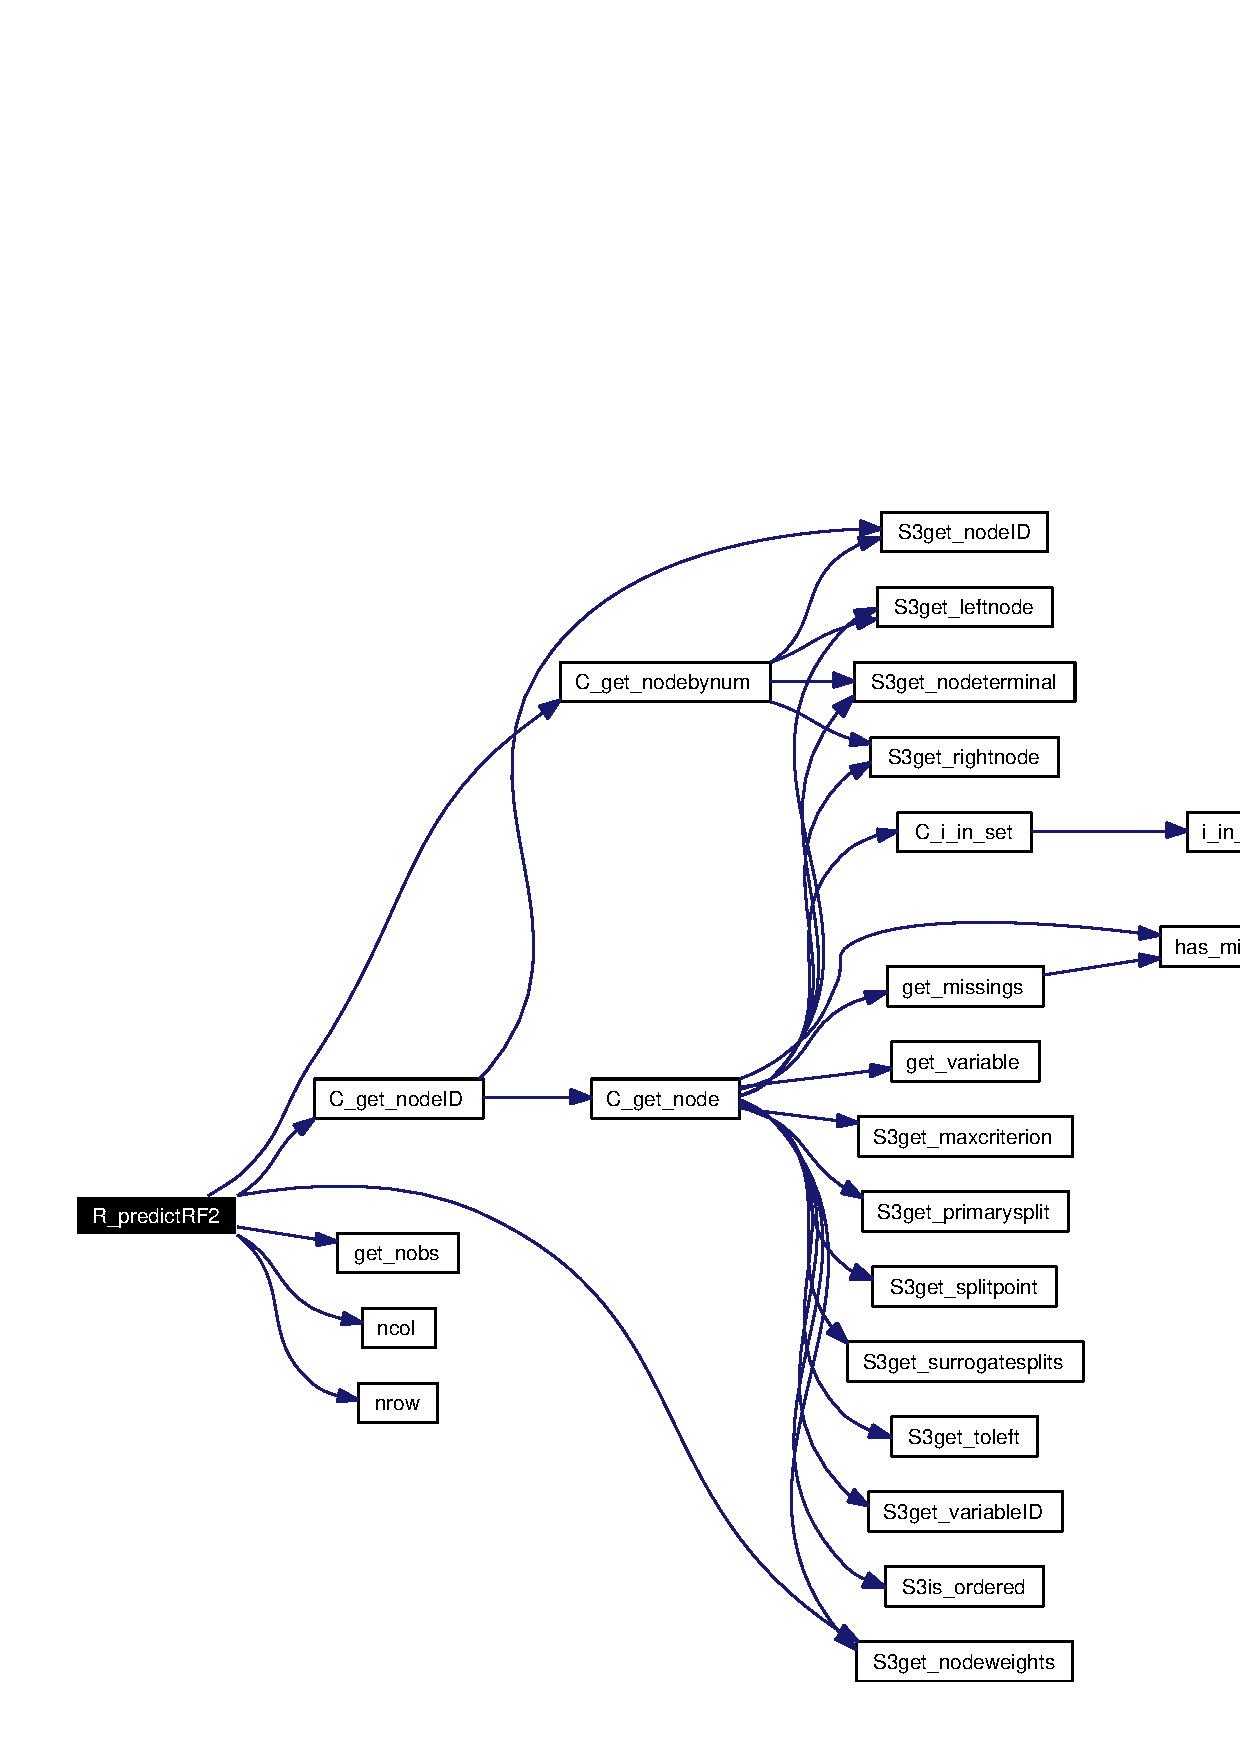
\includegraphics[width=317pt]{Predict_8c_a4f23088af5379408f00d3809656d0da_cgraph}
\end{center}
\end{figure}
\hypertarget{Predict_8c_b1c6e1c0c34af27c7f587b53deb4dc4f}{
\index{Predict.c@{Predict.c}!R_predictRF_weights@{R\_\-predictRF\_\-weights}}
\index{R_predictRF_weights@{R\_\-predictRF\_\-weights}!Predict.c@{Predict.c}}
\subsubsection[R\_\-predictRF\_\-weights]{\setlength{\rightskip}{0pt plus 5cm}SEXP R\_\-predict\-RF\_\-weights (SEXP {\em forest}, SEXP {\em newinputs}, SEXP {\em mincriterion}, SEXP {\em oobpred})}}
\label{Predict_8c_b1c6e1c0c34af27c7f587b53deb4dc4f}


Predictions weights from Random\-Forest objects \begin{Desc}
\item[Parameters:]
\begin{description}
\item[{\em forest}]a list of trees \item[{\em newinputs}]an object of class `Variable\-Frame' \item[{\em mincriterion}]overwrites mincriterion used for tree growing \item[{\em oobpred}]a logical indicating out-of-bag predictions \end{description}
\end{Desc}


Definition at line 639 of file Predict.c.

References C\_\-get\_\-nodebynum(), C\_\-get\_\-node\-ID(), get\_\-nobs(), S3get\_\-nodeweights(), and S3get\_\-prediction().

Here is the call graph for this function:\begin{figure}[H]
\begin{center}
\leavevmode
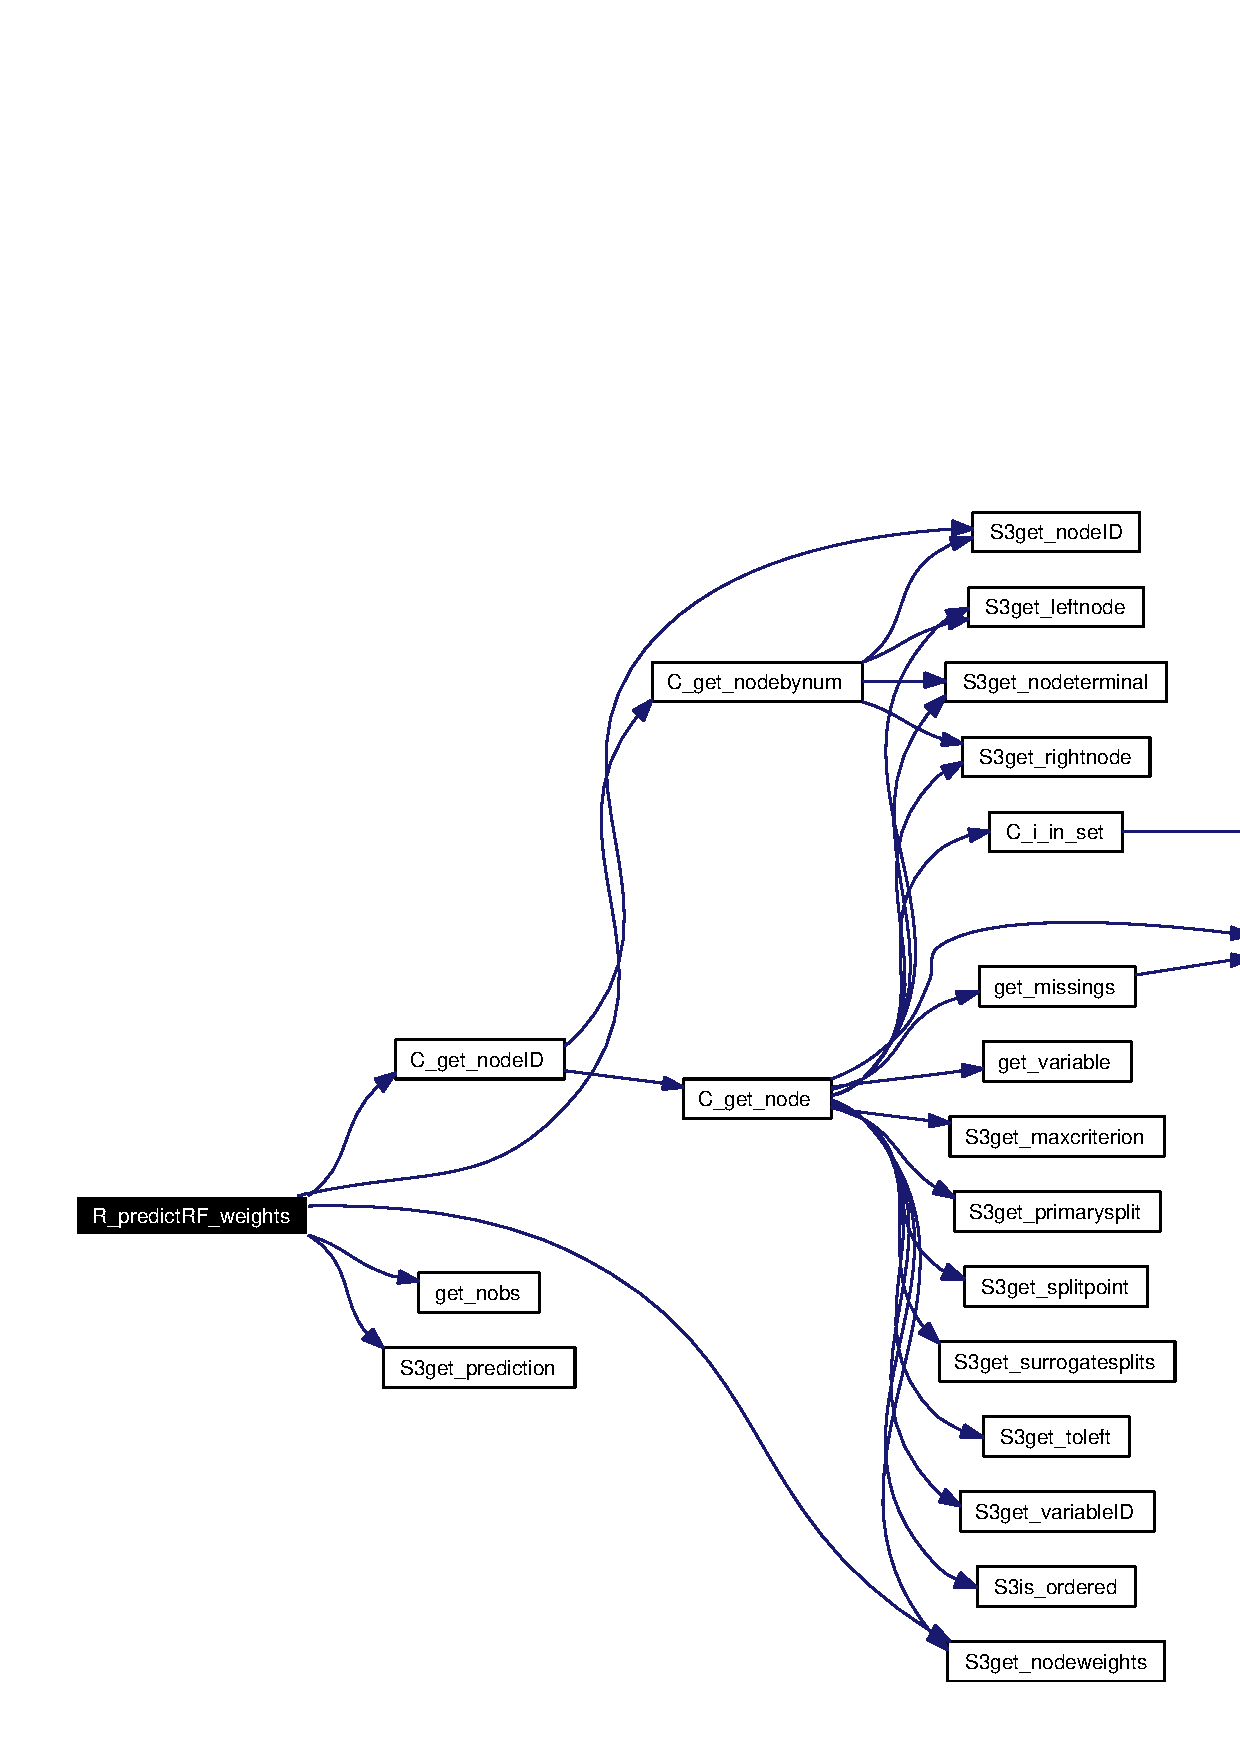
\includegraphics[width=339pt]{Predict_8c_b1c6e1c0c34af27c7f587b53deb4dc4f_cgraph}
\end{center}
\end{figure}
\hypertarget{Predict_8c_0f24ac195825953e630d3386b4d98f97}{
\index{Predict.c@{Predict.c}!R_weights@{R\_\-weights}}
\index{R_weights@{R\_\-weights}!Predict.c@{Predict.c}}
\subsubsection[R\_\-weights]{\setlength{\rightskip}{0pt plus 5cm}SEXP R\_\-weights (SEXP {\em tree}, SEXP {\em newinputs}, SEXP {\em mincriterion})}}
\label{Predict_8c_0f24ac195825953e630d3386b4d98f97}


R-Interface to C\_\-weights \par
 \begin{Desc}
\item[Parameters:]
\begin{description}
\item[{\em tree}]a tree \item[{\em newinputs}]an object of class `Variable\-Frame' \item[{\em mincriterion}]overwrites mincriterion used for tree growing \end{description}
\end{Desc}


Definition at line 497 of file Predict.c.

References C\_\-weights(), and get\_\-nobs().

Here is the call graph for this function:\begin{figure}[H]
\begin{center}
\leavevmode
\includegraphics[width=357pt]{Predict_8c_0f24ac195825953e630d3386b4d98f97_cgraph}
\end{center}
\end{figure}
